
\subsection{Weak error} \label{sec:Weak error plots_no_change}

We start our numerical experiments with estimating accurately the weak error (bias)  for the different parameter sets as in Table \ref{table:Reference solution, using MC with $500$ time steps, of Call option price under rBergomi model, for different parameter constellation.}, with and without Richardson extrapolation.  We consider a number of time steps $N \in \{2,4,8,16\}$. The options are priced in terms of the moneyness.  The reference solution was computed with $N=500$ time steps. We note that the weak errors considered here correspond to relative errors. We show in Table \ref{table:Reference solution, using MC with $500$ time steps, of Call option price under rBergomi model, for different parameter constellation.} the different parameter constellations that we consider to report our results for MC and MISC, along with the corresponding reference solution.


\begin{table}[!h]
	\centering
	\begin{small}
	\begin{tabular}{l*{2}{c}r}
		Parameters            & Reference solution    \\

			Set $1$:	$H=0.07, K=1,S_0=1, \rho=-0.9, \eta=1.9,\xi=0.235^2$   & $\underset{(7.9e-05)}{0.0791}$  \\	

				Set $2$:	$H=0.02, K=1, S_0=1, \rho=-0.7, \eta=0.4,\xi=0.1$   & $\underset{(1.3e-04)}{0.1248}$  \\
					Set $3$:	$H=0.02, K=0.8,S_0=1, \rho=-0.7, \eta=0.4,\xi=0.1$   & $\underset{(5.6e-04)}{0.2407}$  \\
						Set $4$:	$H=0.02, K=1.2,S_0=1, \rho=-0.7, \eta=0.4,\xi=0.1$   & $\underset{(2.5e-04)}{0.0568}$  \\
		\hline
	\end{tabular}
\end{small}
	\caption{Reference solution, using MC with $500$ time steps and number of samples, $M=10^6$, of call option price under the rBergomi model, for different parameter constellations.  The numbers between parentheses correspond to the statistical errors estimates.}
	\label{table:Reference solution, using MC with $500$ time steps, of Call option price under rBergomi model, for different parameter constellation.}
\end{table}





\FloatBarrier

For illustration purposes, we just show the weak errors related to set $1$ in Table \ref{table:Reference solution, using MC with $500$ time steps, of Call option price under rBergomi model, for different parameter constellation.} (see Figure \ref{fig:Weak_rate_set1_set_2_without_rich}). We note that we observed similar behavior for the other parameter sets, with slightly worse rates for some cases.


\begin{figure}[h!]
	\centering
	\begin{subfigure}{.4\textwidth}
		\centering
		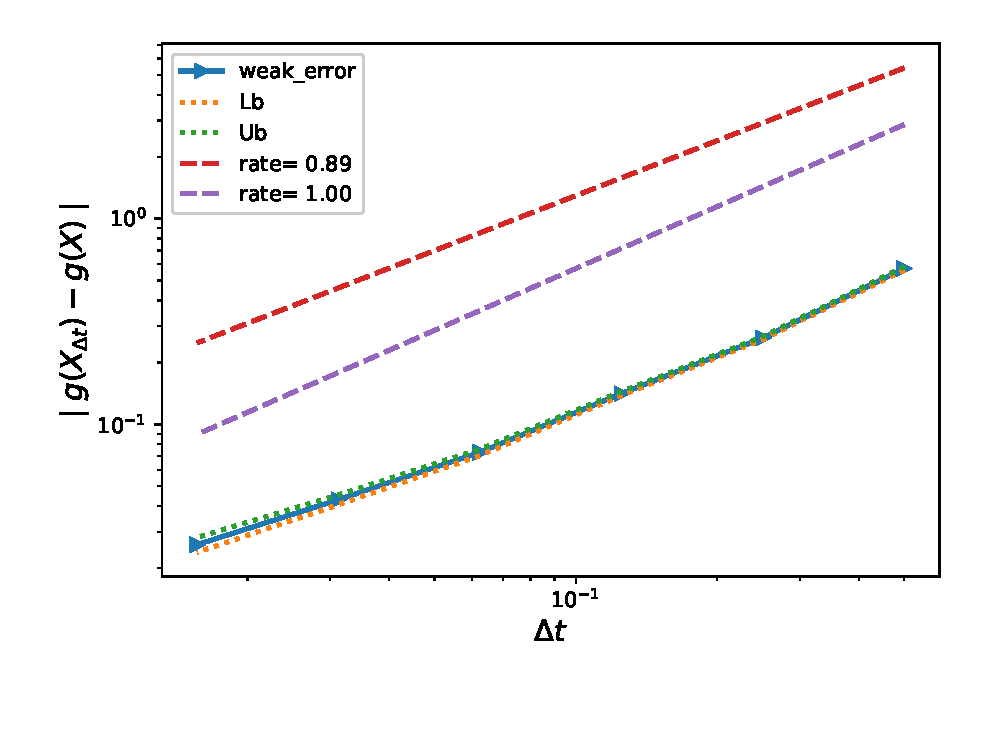
\includegraphics[width=1\linewidth]{./figures/rBergomi_weak_error_rates/without_richardson/H_007/weak_convergence_order_Bergomi_H_007_K_1_M_10_6_CI_relative}
		\caption{}
		\label{fig:sub3}
	\end{subfigure}%
	\begin{subfigure}{.4\textwidth}
		\centering
		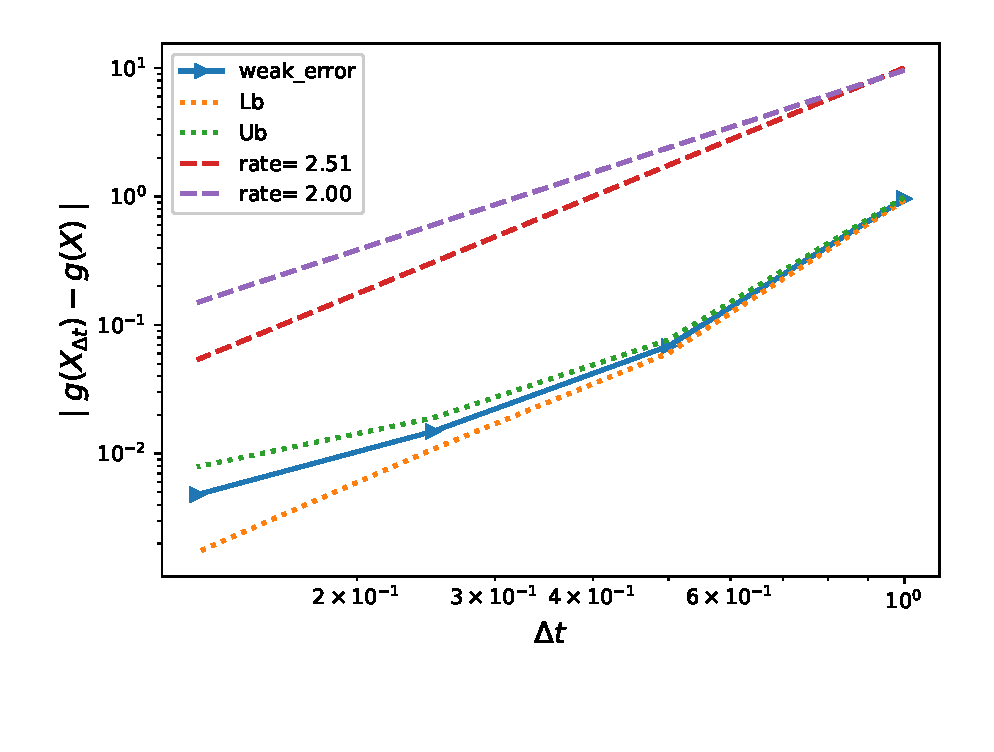
\includegraphics[width=1\linewidth]{./figures/rBergomi_weak_error_rates/with_richardson/H_007/weak_convergence_order_Bergomi_H_007_K_1_richardson_relative_M_10_6}
		\caption{}
		\label{fig:sub4}
	\end{subfigure}
	
	\caption{The  convergence of the weak error, using MC, for set $1$ parameter in Table \ref{table:Reference solution, using MC with $500$ time steps, of Call option price under rBergomi model, for different parameter constellation.}. The upper and lower bounds are $95\%$ confidence intervals. a) Without Richardson extrapolation.  b) With Richardson extrapolation (level $1$).}
	\label{fig:Weak_rate_set1_set_2_without_rich}
\end{figure}
\FloatBarrier




\begin{remark}
We emphasize that the reported weak rates correspond to the pre-asymptotic regime that we are interested in. Our results are purely experimental, and hence we cannot be sure what will happen in the asymptotic regime. We are not interested in estimating the rates specifically but rather obtaining  a sufficiently precise estimate of the weak error (bias), $\mathcal{E}_B(N)$, for different  number of time steps , $N$.  For a fixed discretization, the corresponding biased solution will be set as a reference solution to  MISC method  in order to estimate the quadrature error $\mathcal{E}_Q(\text{TOL}_{\text{MISC}},N)$.	
\end{remark}

%
%\begin{figure}[!htb]
%	\centering
%	\begin{subfigure}{.35\textwidth}
%		\centering
%		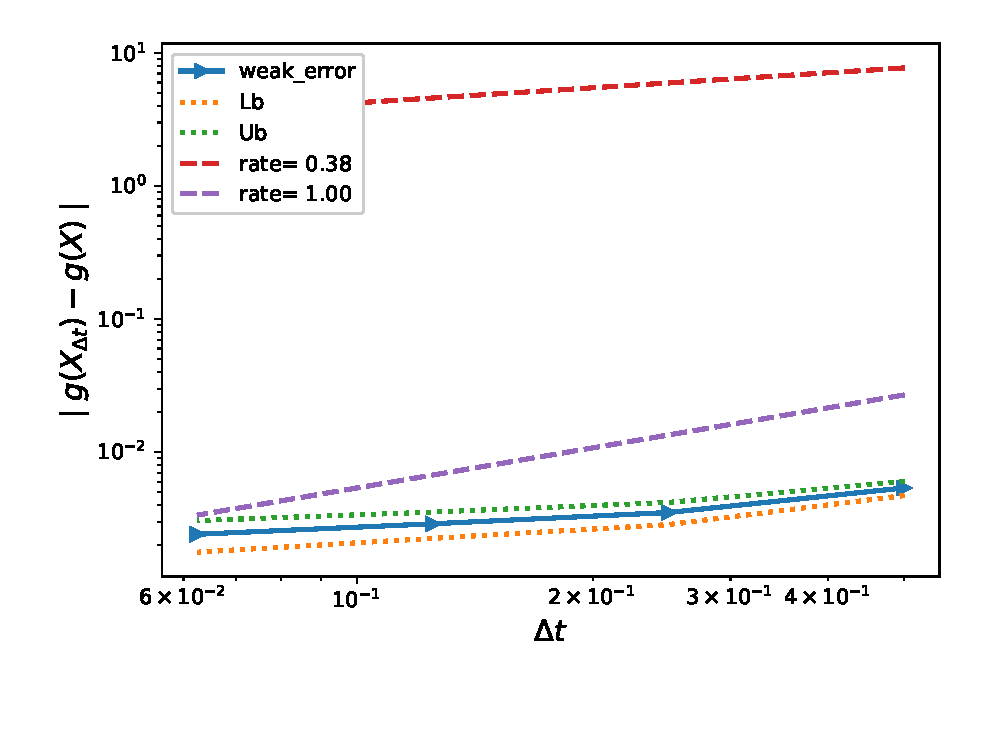
\includegraphics[width=1\linewidth]{./figures/rBergomi_weak_error_rates/without_richardson/H_002/weak_convergence_order_Bergomi_H_002_K_08_M_5_10_6_CI_relative}
%		\caption{}
%		\label{fig:sub3}
%	\end{subfigure}%
%	\begin{subfigure}{.35\textwidth}
%		\centering
%		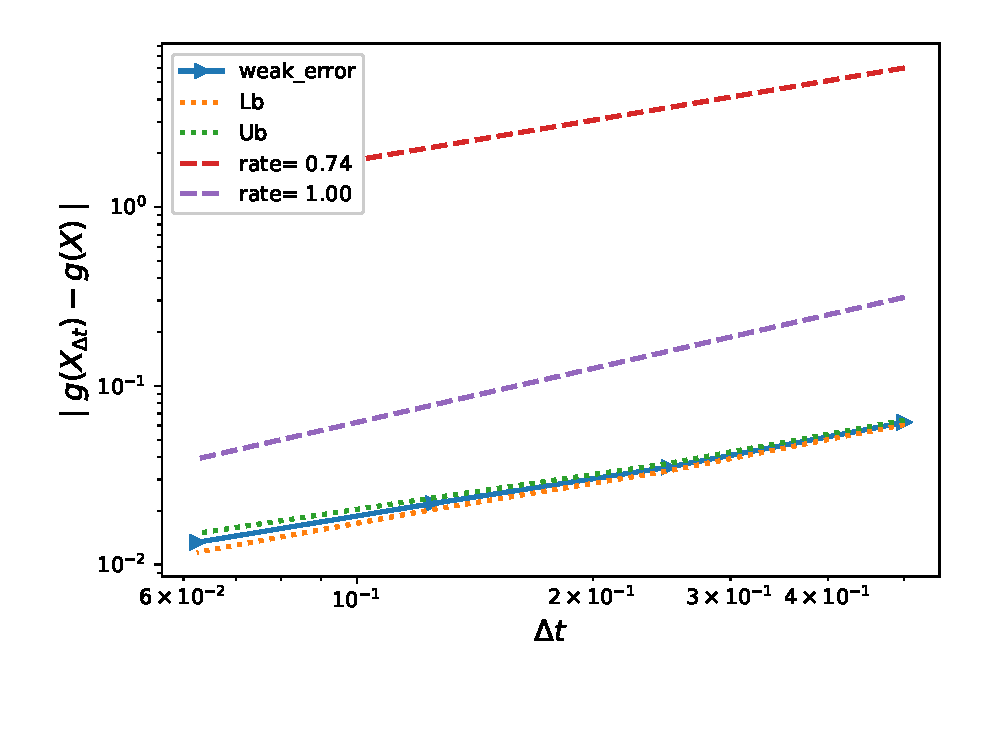
\includegraphics[width=1\linewidth]{./figures/rBergomi_weak_error_rates/without_richardson/H_002/weak_convergence_order_Bergomi_H_002_K_12_M_3_10_6_CI_relative}
%		\caption{}
%		\label{fig:sub4}
%	\end{subfigure}
%	
%	\caption{The rate of convergence of the weak error $\abs{\expt{g(X_{\Delta t})}-g(X)}$  without Richardson extraploation, using MC with $M=5.10^6$: a) Set $3$ parameters in table \ref{table:Reference solution, using MC with $500$ time steps, of Call option price under rBergomi model, for different parameter constellation.},  b) Set $4$ parameters in table \ref{table:Reference solution, using MC with $500$ time steps, of Call option price under rBergomi model, for different parameter constellation.}. }
%	\label{fig:Weak_rate_H_002_without_rich_K_1_K_08}
%\end{figure}

\FloatBarrier









%\begin{figure}[!htb]
%		\centering
%		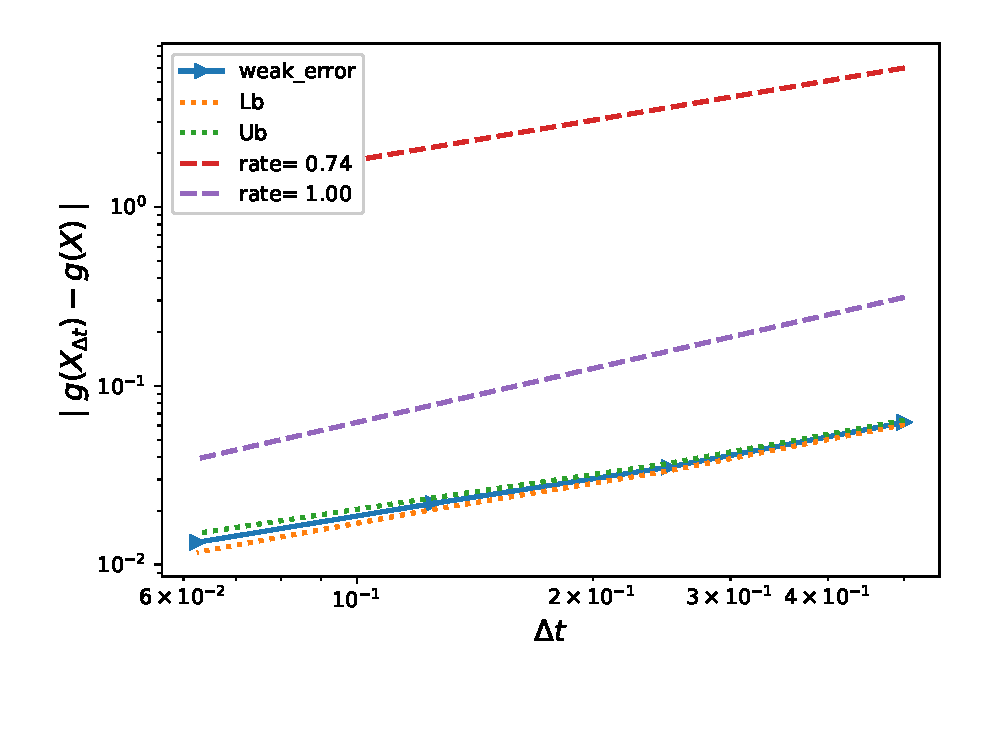
\includegraphics[width=0.35\linewidth]{./figures/rBergomi_weak_error_rates/without_richardson/H_002/weak_convergence_order_Bergomi_H_002_K_12_M_3_10_6_CI_relative}	
%	\caption{The rate of convergence of the weak error $\abs{\expt{g(X_{\Delta t})}-g(X)}$, for set $5$ parameters in table \ref{table:Reference solution, using MC with $500$ time steps, of Call option price under rBergomi model, for different parameter constellation.}, without Richardson extraploation, using MC with $M=5.10^6$.}
%	\label{fig:Weak_rate_H_002_without_rich_K_12}
%\end{figure}




%\subsubsection{With Richardson extrapolation (level 1)}

%\FloatBarrier
%\begin{figure}[h!]
%	\centering
%	\begin{subfigure}{.35\textwidth}
%		\centering
%		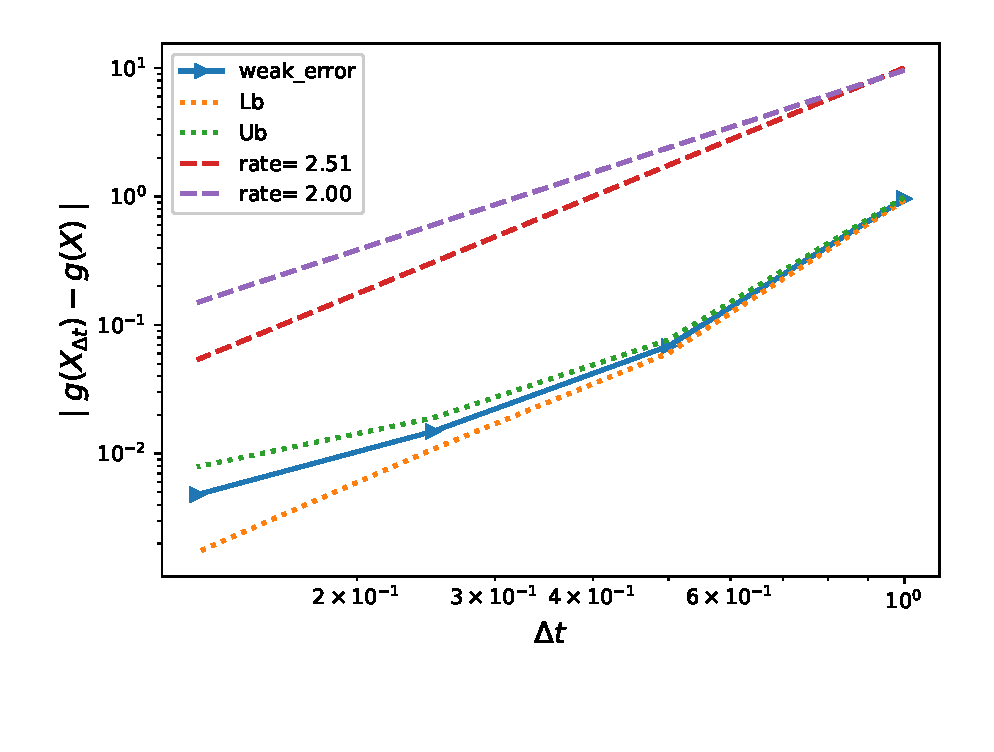
\includegraphics[width=1\linewidth]{./figures/rBergomi_weak_error_rates/with_richardson/H_007/weak_convergence_order_Bergomi_H_007_K_1_richardson_relative_M_10_6}
%		\caption{}
%		\label{fig:sub3}
%	\end{subfigure}%
%	\begin{subfigure}{.35\textwidth}
%		\centering
%		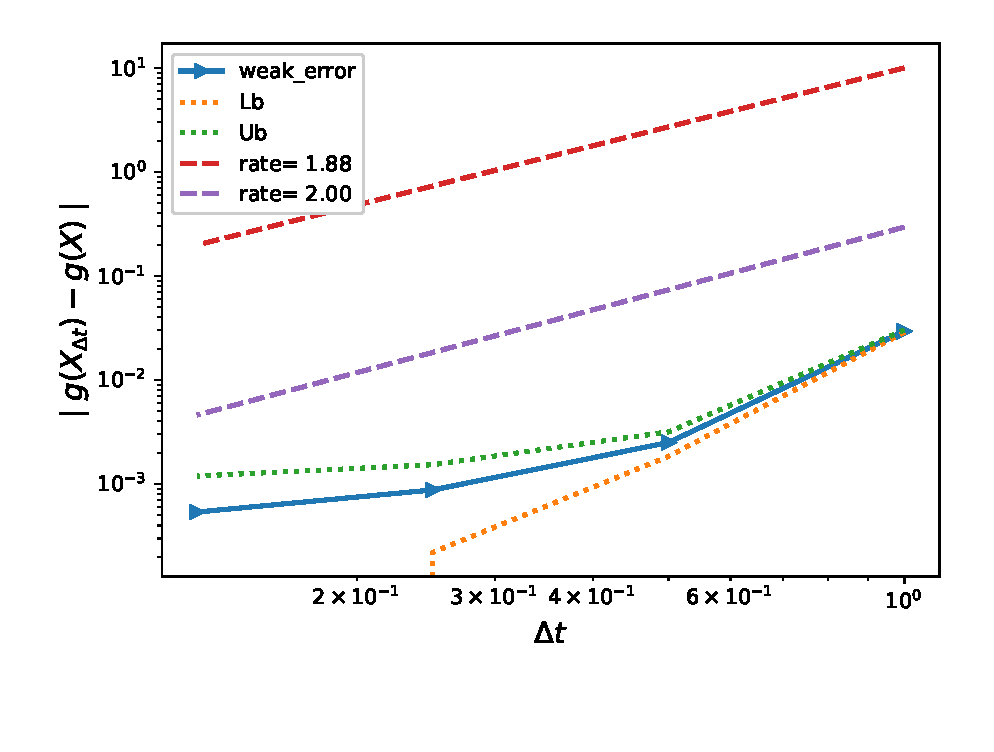
\includegraphics[width=1\linewidth]{./figures/rBergomi_weak_error_rates/with_richardson/H_002/weak_convergence_order_Bergomi_H_002_K_1_M_1_10_7_richardson_relative}
%		\caption{}
%		\label{fig:sub4}
%	\end{subfigure}
%	
%	\caption{The rate of convergence of the weak error  $\abs{\expt{2 g(X_{\Delta t/2}) -g(X_{\Delta t})}-g(X)}$   with Richardson extraploation, using MC with $M=10^6$: a) Set $1$ parameters in table \ref{table:Reference solution, using MC with $500$ time steps, of Call option price under rBergomi model, for different parameter constellation.}.  b) Set $2$ parameters in table \ref{table:Reference solution, using MC with $500$ time steps, of Call option price under rBergomi model, for different parameter constellation.}, }
%	\label{fig:Weak_rate_H_043_007_with_rich}
%\end{figure}
%
%
\FloatBarrier

%\begin{figure}[!htbp]
%	\centering
%		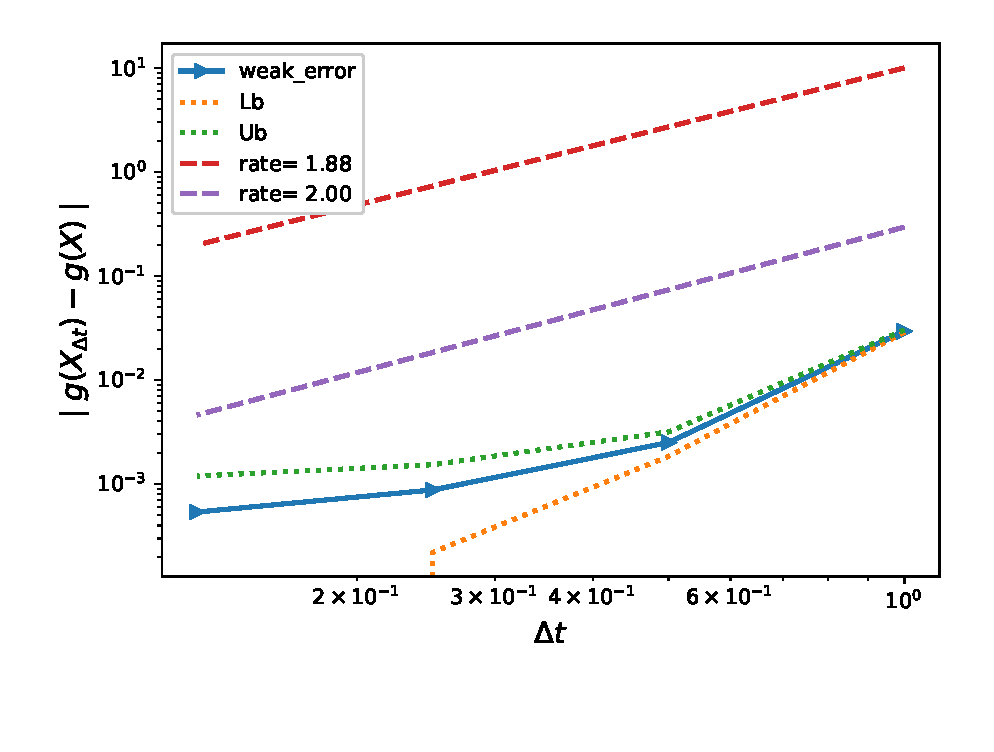
\includegraphics[width=0.35\linewidth]{./figures/rBergomi_weak_error_rates/with_richardson/H_002/weak_convergence_order_Bergomi_H_002_K_1_M_1_10_7_richardson_relative}
%	\caption{The rate of convergence of the weak error $\abs{\expt{2 g(X_{\Delta t/2}) -g(X_{\Delta t})}-g(X)}$,  for set $3$ parameters in table \ref{table:Reference solution, using MC with $500$ time steps, of Call option price under rBergomi model, for different parameter constellation.}, with Richardson extraploation, using MC with $M=10^7$. }
%	\label{fig:Weak_rate_H_002_with_rich_K1}
%\end{figure}
%\FloatBarrier



\red{
\subsection{Comparing the different  errors and computational time for MC and MISC}\label{sec:Comparing different  errors and complexity for MC and MISC}



In this Section, we conduct a comparison between MC and MISC in terms of errors and computational time. we show tables and plots reporting  the different relative errors involved in MC method (bias and statistical error), and in MISC (bias and quadrature error).  Fixing a  sufficiently small error tolerance in the price estimates,  we also compare the computational time needed for both methods to meet the desired error tolerance. The results are reported for the different sets of parameters defined in Table \ref{table:Reference solution, using MC with $500$ time steps, of Call option price under rBergomi model, for different parameter constellation.}, and we consider   a number of time steps $N \in \{2,4,8,16\}$.  The options are priced in terms of the moneyness.  We emphasize that all reported errors are relative errors normalized by the reference solutions provided in Table \ref{table:Reference solution, using MC with $500$ time steps, of Call option price under rBergomi model, for different parameter constellation.}. We also note that  in all cases the actual work (runtime) is obtained using an Intel(R) Xeon(R) CPU E$5$-$268$ architecture. 


Through our conducted numerical experiments for each parameter set, we follow these steps to get our reported results:

\begin{enumerate}
\item[i)] For a fixed number of time steps, $N$, we compute an accurate estimate, using a large number of samples, $M$, of the biased  MC solution, $C_{RB}^{N}$. This step also provide us with the bias error, $\mathcal{E}_B(N)$, defined by \eqref{eq:total_error}. 
\item[ii)] The estimated  biased solution,  $C_{RB}^{N}$, is used as a reference solution  to MISC to compute the quadrature error, $\mathcal{E}_Q(\text{TOL}_{\text{MISC}},N)$, defined by \eqref{eq:quadrature error}. Although we report the quadrature error for different MISC tolerances, $\text{TOL}_{\text{MISC}}$, we just pick the asymptotic value of the quadrature error, given by MISC, to be used for comparison purposes against MC.

\item[iii)]  Given that both methods, MC and MISC, have the same bias error,  the computational time of MC and MISC is compared such that the statistical error estimate \footnote{The statistical error estimate of MC is  $\frac{\sigma_M}{\sqrt{M}}$, where $M$ is the number of samples and $\sigma_M$ is the standard deviation estimate of the MC estimator.} is almost equal to the asymptotic quadrature error of MISC. 
\end{enumerate}

We show in Table \ref{table:Summary of our numerical results.} the summary of our numerical findings, highlighting the substantial computational gains achieved by MISC over MC to meet a certain error tolerance. More detailed results for each case of parameter set, as in Table \ref{table:Reference solution, using MC with $500$ time steps, of Call option price under rBergomi model, for different parameter constellation.},  are provided in  Sections (\ref{sec:Case of set $2$ parameters_linear}, \ref{sec:Case of set 3 parameters}, \ref{sec:Case of set 4 parameters}, \ref{sec:Case of set 5 parameters}). 



\FloatBarrier
\begin{table}[!h]
	\centering
	\begin{small}
	\begin{tabular}{l*{4}{c}r}
		Parameter set           & Level of Richardson extrapolation    &  Total relative error  & Ratio of CPU time  $\left(\text{MC}/ \text{MISC} \right)$ \\
			Set $1$ & level $1$ &  $2.5\%$&  $3.5$ \\	
              & level $2$ &  $0.9\%$ &  $17$ \\	
              \hline
            Set $2$  & without    &  $0.5\%$&  $18$ \\	
				 & level $1$ &  $0.2\%$&  $20$ \\	
				 \hline
					Set $3$  & without    &  $0.4\%$&  $41$ \\	
					\hline
						Set $4$ & without  &  $2\%$&  $16$ \\	
		\hline
	\end{tabular}
\end{small}
	\caption{Summary of our numerical results.}
	\label{table:Summary of our numerical results.}
\end{table}


\FloatBarrier

	
	



%\subsubsection{Case of set $1$ parameters in table \ref{table:Reference solution, using MC with $500$ time steps, of Call option price under rBergomi model, for different parameter constellation.}}\label{sec:Case of set 1 parameters}
%
%\subsubsection*{Without Richardson extrapolation}
%%\begin{table}[h!]
%%	\centering
%%	\begin{tabular}{l*{6}{c}r}
%%		Method \textbackslash  Steps            & $2$ & $4$ & $8$ & $16$ &   \\
%%		\hline
%%%		MISC ($\text{TOL}_{\text{MISC}}=5.10^{-1}$)  & $0.1140$ & $0.0961$ & $0.0848$ & $0.0781$  \\
%%		MISC ($\text{TOL}_{\text{MISC}}=10^{-1}$)  & $0.1140$ & $0.0961$ & $0.0871$ & $0.0802$  \\
%%%		MISC ($\text{TOL}_{\text{MISC}}=5.10^{-2}$)  & $0.1140$ & $0.0963$ & $0.0843$ & $0.0824$  \\
%%		MISC ($\text{TOL}_{\text{MISC}}=10^{-2}$)  & $0.1077$ & $0.0944$ & $0.0838$ & $0.0772$  \\
%%
%%		MISC ($\text{TOL}_{\text{MISC}}=10^{-3}$)  & $0.1077$ & $0.0921$ & $0.0819$ & $0.0762$  \\
%%%		MISC ($\text{TOL}_{\text{MISC}}=5.10^{-4}$)  & $0.1079   $ & $0.0921$ & $0.0822$ & $0.0762$  \\
%%		MISC ($\text{TOL}_{\text{MISC}}=10^{-4}$)  & $0.1079$ & $0.0921$ & $0.0822$ & $-$  \\
%%		\hline
%%		MC method ($M=8.10^{6}$)   & $  0.1078$ & $ 0.0921
%%		$  & $   0.0822
%%		$ & $ 0.0767$ \\		
%%		
%%		\hline
%%	\end{tabular}
%%	\caption{ Call option price of the different methods for different number of time steps. Case of set $1$ parameters in table \ref{table:Reference solution, using MC with $500$ time steps, of Call option price under rBergomi model, for different parameter constellation.}, without Richardson extrapolation.}
%%	\label{table: Call option price of the different methods for different number of time steps. Case set 1}
%%\end{table}
%
%
%\begin{table}[h!]
%	\centering
%	\begin{tabular}{l*{6}{c}r}
%		Method \textbackslash  Steps            & $2$ & $4$ & $8$ & $16$  \\
%		\hline
%		MC Bias ($M=8.10^6$)   & 	$ \underset{( 0.0366)}{\mathbf{0.5142}}$  & $\underset{( 0.0209)}{\mathbf{0.2933}}$  & $\underset{( 0.0110)}{\mathbf{0.1551}}$ & $\underset{( 0.0055)}{\mathbf{0.0777}}$\\ 
%		
%		MC Statistical error ($M=8.10^6$)  &  $\underset{(  6.0e-05)} {\mathbf{8.4e-04}}$  & $\underset{(3.4e-05)} {\mathbf{4.8e-04}}$  & $\underset{(2.7e-05)} {\mathbf{ 3.8e-04}}$ & $\underset{( 2.35e-05)} {\mathbf{3.3e-04}}$	\\
%
%		\hline
%	\end{tabular}
%	\caption{Bias and statistical errors of MC  for computing call option price  for different number of time steps. Case set $1$, without Richardson extrapolation. The numbers between parentheses are the corresponding absolute errors.}
%	\label{Bias and Statistical errors of MC ($M=10^6$)  for computing Call option price  for different number of time steps. Case set 1, without Richardson extrapolation. The numbers between parentheses are the corresponding absolute errors.}
%\end{table}
%
%
%
%
%
%
%\FloatBarrier
%
%\begin{figure}[h!]
%	\centering
%	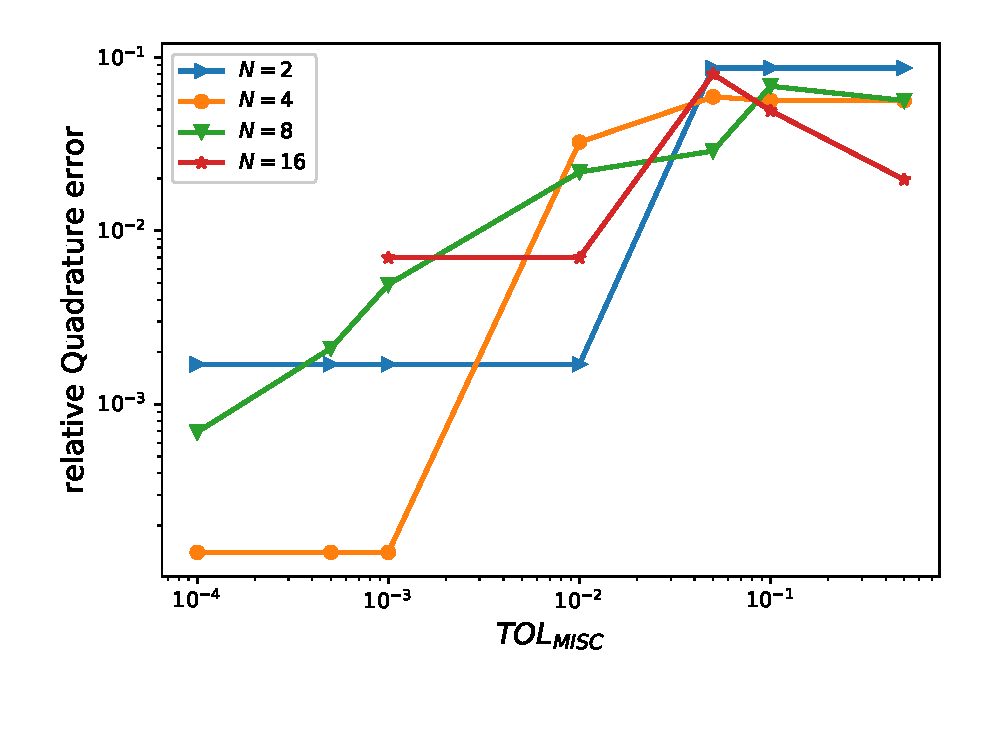
\includegraphics[width=0.35\linewidth]{./figures/rBergomi_MISC_quadratre_error/vs_TOL/set1/relative_quad_error_wrt_MISC_TOL_set1_non_rich}
%	
%	
%	\caption{Quadrature error of MISC, with different tolerances, to compute call option price for different number of time steps. Case  set $1$ parameters, without Richardson extrapolation. See detailed values  in table \ref{Quadrature error of MISC to compute Call option price of the different tolerances for different number of time steps. Case  set $1$ parameters, without Richardson extrapolation. The numbers between parentheses are the corresponding absolute errors.}}
%	\label{fig:Quadrature_error_set1}
%\end{figure}
%
%\FloatBarrier
%
%
%\begin{table}[h!]
%	\centering
%	\begin{tabular}{l*{6}{c}r}
%		Method \textbackslash  Steps            & $2$ & $4$ & $8$ & $16$  \\
%		\hline
%%		MISC ($\text{TOL}_{\text{MISC}}=5.10^{-1}$)  & $\mathbf{0.6010}$ & $\mathbf{0.3496}$ & $\mathbf{ 0.2114}$ & $\mathbf{ 0.0974}$  \\
%		MISC ($\text{TOL}_{\text{MISC}}=10^{-1}$)  & $\mathbf{0.6010}$ & $\mathbf{0.3496}$ & $\mathbf{  0.2232}$ & $\mathbf{
%			0.1269}$  \\
%%		MISC ($\text{TOL}_{\text{MISC}}=5.10^{-2}$)  &$\mathbf{0.6010}$ & $\mathbf{  0.3524}$ & $\mathbf{ 0.1839}$ & $\mathbf{  0.1577}$  \\
%		MISC ($\text{TOL}_{\text{MISC}}=10^{-2}$)  & $\mathbf{\red{0.5159}}$ & $\mathbf{0.3257}$ & $\mathbf{ 0.1769}$ & $\mathbf{  \red{0.0847}}$  \\
%		MISC ($\text{TOL}_{\text{MISC}}=10^{-3}$)  & $\mathbf{0.5159}$ & $\mathbf{\red{0.2934}}$ & $\mathbf{0.1600}$ & $\mathbf{0.0847}$  \\
%%		MISC ($\text{TOL}_{\text{MISC}}=5.10^{-4}$)  & $\mathbf{0.5159}$ & $\mathbf{0.2934}$ & $\mathbf{0.1572}$ & $\mathbf{-}$  \\
%		MISC ($\text{TOL}_{\text{MISC}}=10^{-4}$)  & $\mathbf{0.5159}$ & $\mathbf{0.2934}$ & $\mathbf{\red{0.1558}}$ & $\mathbf{-}$  \\
%		\hline
%		MC     & $\mathbf{\red{0.5159}}$ & $\mathbf{\red{0.2938}}$ & $\mathbf{\red{0.1555}}$ &$\mathbf{  \red{0.0817}}$  \\	
%		
%		\hline
%	\end{tabular}
%	\caption{Total relative error of MISC, with different tolerances,  and MC to compute call option price for different number of time steps. Case  set $1$ parametrs of table \ref{table:Reference solution, using MC with $500$ time steps, of Call option price under rBergomi model, for different parameter constellation.}, without Richardson extrapolation. The values marked in red, for MISC method, correspond to the total relative errors associated with  stable quadrature errors for MISC, and will be used for complexity comparison against MC.}
%	\label{Total error of MISC and MC to compute Call option price of the different tolerances for different number of time steps. Case set 1, without Richardson extrapolation. The numbers between parentheses are the corresponding absolute errors.}
%\end{table}
%
%
%
%\begin{table}[h!]
%	\centering
%	\begin{tabular}{l*{6}{c}r}
%		Method \textbackslash  Steps            & $2$ & $4$ & $8$ & $16$ &   \\
%		\hline
%%		MISC ($\text{TOL}_{\text{MISC}}=5.10^{-1}$)  & $0.1$ & $0.1$ & $0.2$ & $0.4$  \\
%		MISC ($\text{TOL}_{\text{MISC}}=10^{-1}$)  & $0.1$ & $0.1$ & $0.6$ & $6$  \\
%%		MISC ($\text{TOL}_{\text{MISC}}=5.10^{-2}$)  & $0.1$ & $0.3$ & $2$ & $14$  \\
%		MISC ($\text{TOL}_{\text{MISC}}=10^{-2}$)  & $\red{0.2}$ & $1$ & $9$ & $\red{215}$  \\
%		MISC ($\text{TOL}_{\text{MISC}}=10^{-3}$)  & $2$ & $\red{11}$ & $243$ & $4650$  \\
%%		MISC ($\text{TOL}_{\text{MISC}}=5.10^{-4}$)  & $3$ & $17$ & $ 670$ & $-$  \\
%		MISC ($\text{TOL}_{\text{MISC}}=10^{-4}$)  & $6$ & $96$ & $\red{5760}$ & $-$  \\
%		\hline
%		MC     & $\red{ 50}$  & $\red{344}$  & $\red{637}$ & $\red{8}$  \\
%		
%		\hline
%		Ratio of $\left(\text{MC}/ \text{MISC} \right)$  &$\red{  250}$ & $\red{    31
%		}$  & $\red{ 0.1
%		}$  & $\red{  0.04}$ \\
%		\hline
%	\end{tabular}
%	\caption{Comparison of the computational time (in Seconds) of  MC and MISC, used to compute call option price of the rBergomi model for different number of time steps. Case set $1$ parametrs of table \ref{table:Reference solution, using MC with $500$ time steps, of Call option price under rBergomi model, for different parameter constellation.}. The
%		average MC CPU time is computed over 10 runs. }
%	\label{Comparison of the computational time of  MC and MISC, used to compute Call option price of rBergomi model for different number of time steps. Case set1}
%\end{table}
%
%\FloatBarrier
%\subsubsection*{With Richardson extrapolation (level $1$)}
%
%
%
%
%
%
%
%%\begin{table}[h!]
%%	\centering
%%	\begin{tabular}{l*{6}{c}r}
%%		Method \textbackslash  Steps    &$1-2$         & $2-4$ & $4-8$ \\
%%		\hline
%%%		MISC ($\text{TOL}_{\text{MISC}}=5.10^{-1}$)& $0.1357$  & $0.0783$ & $0.0735$ \\
%%		MISC ($\text{TOL}_{\text{MISC}}=10^{-1}$)  &$0.1357$  &$0.0783$ & $0.0785$   \\
%%%		MISC ($\text{TOL}_{\text{MISC}}=5.10^{-2}$)  & $0.1357$ & $0.0831$ & $0.0773$   \\
%%		MISC ($\text{TOL}_{\text{MISC}}=10^{-2}$)  & $0.1237$ &$0.0781$ & $0.0745$   \\
%%
%%		MISC ($\text{TOL}_{\text{MISC}}=10^{-3}$)  & $0.1224$ &$0.0766$ & $0.0720$  \\
%%%		MISC ($\text{TOL}_{\text{MISC}}=10^{-4}$)  &$0.1224$ & $0.0763$ & $0.0724$ \\
%%		\hline
%%		MC method ($M=10^6$)  &$	0.1237$ & $0.0752$ & $0.0721$ \\
%%		\hline
%%	\end{tabular}
%%	\caption{Call option price of the different methods for different number of time steps. Case set $1$ parameters of table \ref{table:Reference solution, using MC with $500$ time steps, of Call option price under rBergomi model, for different parameter constellation.}, using Richardson extrapolation (level $1$).}
%%	\label{table:  Call option price of the different methods for different number of time steps. Case set $1$ parameter, using Richardson extrapolation (level $1$)}
%%\end{table}
%
%
%
%
%\begin{table}[h!]
%	\centering
%	\begin{tabular}{l*{6}{c}r}
%		Method \textbackslash  Steps            & $1-2$ & $2-4$ & $4-8$ & $8-16$  \\
%		\hline
%		MC  Bias ($M=10^6$)    &$\underset{( 0.0525)}{\mathbf{0.7378}}$  & $\underset{(    0.0040)}{\mathbf{0.0561}}$  & $\underset{(0.0009 )}{\mathbf{0.0127}}$  & $\underset{(0.0001)}{\mathbf{0.0021}}$ \\	
%		
%		MC Statistical error ($M=10^6$)   & $\underset{( 2.3e-04)}{\mathbf{3.3e-03}}$  & $\underset{(  1.1e-04)}{\mathbf{1.6e-03}}$  & $\underset{(7.1e-05)}{\mathbf{1.0e-03}}$ & $\underset{(   6.4e-05 )}{\mathbf{9.0e-04}}$ \\	
%		
%		
%		\hline
%	\end{tabular}
%	\caption{Bias and statistical errors of MC   for computing call option price  for different number of time steps. Case set $1$ parameters in tabel \ref{table:Reference solution, using MC with $500$ time steps, of Call option price under rBergomi model, for different parameter constellation.}, with Richardson extrapolation (level $1$). The numbers between parentheses are the corresponding absolute errors.}
%	\label{Bias and Statistical errors of MC ($M=10^6$)  for computing Call option price  for different number of time steps. Case set $1$ parameters, with Richardson extrapolation (level1). The numbers between parentheses are the corresponding absolute errors.}
%\end{table}
%
%
%
%
%
%
%
%
%\begin{figure}[h!]
%	\centering
%	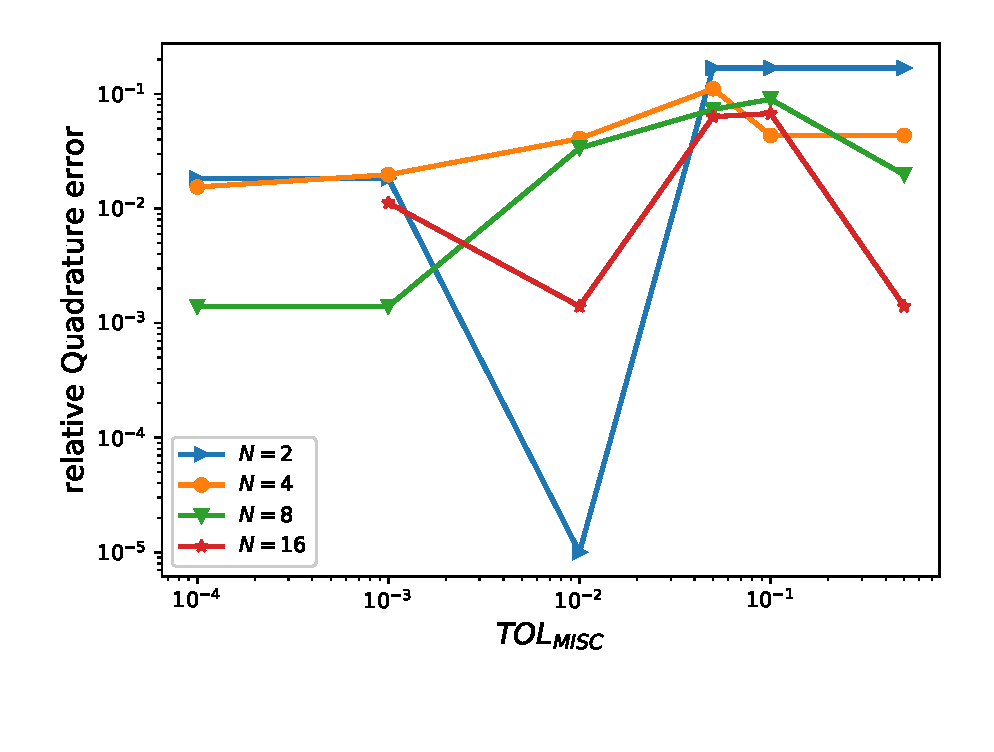
\includegraphics[width=0.35\linewidth]{./figures/rBergomi_MISC_quadratre_error/vs_TOL/set1/relative_quad_error_wrt_MISC_TOL_set1_with_rich}
%	
%	
%	\caption{Quadrature error of MISC, with different tolerances, to compute call option price for different number of time steps. Case  set $1$ parameters, with Richardson extrapolation.  See detailed values  in table \ref{Quadrature error of MISC to compute Call option price of the different tolerances for different number of time steps. Case set $1$ parameters, with Richardson extrapolation(level $1$). The numbers between parentheses are the corresponding absolute errors.}.}
%\end{figure}
%
%
%
%\begin{table}[!h]
%	\centering
%	\begin{tabular}{l*{6}{c}r}
%		Method \textbackslash  Steps            & $1-2$ & $2-4$ & $4-8$   \\
%		\hline
%%		MISC ($\text{TOL}_{\text{MISC}}=5.10^{-1}$)  & $\mathbf{0.9063
%%		}$ & $\mathbf{ 0.0996}$ & $\mathbf{0.0324
%%		}$  \\
%		MISC ($\text{TOL}_{\text{MISC}}=10^{-1}$)  & $\mathbf{0.9063
%		}$ & $\mathbf{ 0.0996}$ & $\mathbf{  0.1026}$   \\
%%		MISC ($\text{TOL}_{\text{MISC}}=5.10^{-2}$)  & $\mathbf{0.9063
%%		}$ & $\mathbf{    0.1670}$ & $\mathbf{ 0.0857}$  \\
%		MISC ($\text{TOL}_{\text{MISC}}=10^{-2}$)  & $\mathbf{0.7378}$ & $\mathbf{  0.0968}$ & $\mathbf{   0.0464}$  \\	
%		MISC ($\text{TOL}_{\text{MISC}}=10^{-3}$)  & $\mathbf{\red{0.7561}}$ & $\mathbf{\red{0.0758}}$ & $\mathbf{\red{0.0141}}$  \\
%%		MISC ($\text{TOL}_{\text{MISC}}=10^{-4}$)  & $\mathbf{0.7561}$ & $\mathbf{0.0715}$ & $\mathbf{0.0141}$ \\
%		\hline
%		MC   & $\mathbf{\red{0.7561}}$  & $\mathbf{\red{0.0758}}$  & $\mathbf{\red{0.0141}}$  \\
%		
%		\hline
%	\end{tabular}
%	\caption{Total  relative error of MISC and MC, with different tolerances, to compute call option price for different number of time steps. Case set $1$ parameters in table \ref{table:Reference solution, using MC with $500$ time steps, of Call option price under rBergomi model, for different parameter constellation.}, with Richardson extrapolation(level $1$). The values marked in red, for MISC method, correspond to the total relative errors associated with  stable quadrature errors for MISC, and will be used for complexity comparison against MC.}
%	\label{Total  error of MISC and MC to compute Call option price of the different tolerances for different number of time steps. Case set $1$ parameters, with Richardson extrapolation(level $1$). The numbers between parentheses are the corresponding absolute errors.}
%\end{table}
%\FloatBarrier
%\begin{table}[!h]
%	\centering
%	\begin{tabular}{l*{6}{c}r}
%		Method \textbackslash  Steps            & $1-2$ & $2-4$ & $4-8$   \\
%		\hline
%%		MISC ($\text{TOL}_{\text{MISC}}=5.10^{-1}$)  & $0.1$ & $0.1$ & $0.2$  \\
%		MISC ($\text{TOL}_{\text{MISC}}=10^{-1}$)  & $0.1$ & $0.1$ & $0.6$ \\
%%		MISC ($\text{TOL}_{\text{MISC}}=5.10^{-2}$)  & $0.1$ & $0.4$ & $2$   \\
%		MISC ($\text{TOL}_{\text{MISC}}=10^{-2}$)  & $1$ & $2$ & $18$   \\
%		MISC ($\text{TOL}_{\text{MISC}}=10^{-3}$)  & $\red{4}$ & $\red{12}$ & $\red{520}$   \\	
%%		MISC ($\text{TOL}_{\text{MISC}}=10^{-4}$)  & $7$ & $191$ & $7650$  \\
%		\hline
%		MC   & $\red{ 34.7}$  & $\red{37}$  & $ \red{532}$    \\
%		
%		\hline
%		Ratio of $\left(\text{MC}/ \text{MISC} \right)$  &$\red{8.7}$ & $\red{   3.1
%		}$  & $\red{1}$ \\
%		\hline
%	\end{tabular}
%	\caption{Comparison of the computational time (in Seconds) of  MC and MISC, using Richardson extrapolation (level $1$), used to compute call option price of the rBergomi model for different number of time steps. Case set $1$ parameters in table \ref{table:Reference solution, using MC with $500$ time steps, of Call option price under rBergomi model, for different parameter constellation.}. The
%		average MC CPU time is computed over 10 runs.}
%	\label{Comparsion of the computational time of  MC and MISC, using Richardson extrapolation (level $1$), used to compute Call option price of rBergomi model for different number of time steps. Case set $1$ parameters}
%\end{table}
%
%
%
%
%\FloatBarrier
%
%\subsubsection*{With Richardson extrapolation (level $2$)}
%%\FloatBarrier
%%\begin{table}[h!]
%%	\centering
%%	\begin{tabular}{l*{6}{c}r}
%%		Method \textbackslash  Steps           &$1-2-4$ & $2-4-8$ \\
%%		\hline
%%%		MISC ($\text{TOL}_{\text{MISC}}=5.10^{-1}$)& $0.0591$  & $0.0719$ \\
%%		
%%		MISC ($\text{TOL}_{\text{MISC}}=10^{-1}$)  &$0.0567$  &$0.0747$   \\
%%%		MISC ($\text{TOL}_{\text{MISC}}=5.10^{-2}$)  & $0.0733$ & $0.0782$  \\
%%		MISC ($\text{TOL}_{\text{MISC}}=10^{-2}$)  & $		0.0639$ & $0.0729$   \\
%%		MISC ($\text{TOL}_{\text{MISC}}=5.10^{-3}$)  & $	0.0620$ & $0.0708$   \\
%%%		MISC ($\text{TOL}_{\text{MISC}}=10^{-3}$)  & $	0.0608$ & $0.0708$  \\
%%%		MISC ($\text{TOL}_{\text{MISC}}=10^{-4}$)  & $	0.0608$ & $-$   \\
%%		\hline
%%		MC ($M=3.10^6$)  & $0.0608$ & $0.0710$   \\
%%		\hline 
%%	\end{tabular}
%%	\caption{ Call option price of the different methods for different number of time steps.  Case set $1$ parameters in table \ref{table:Reference solution, using MC with $500$ time steps, of Call option price under rBergomi model, for different parameter constellation.}, using Richardson extrapolation (level $2$).}
%%	\label{table: Call option price of the different methods for different number of time steps. Case $K=1$, using Richardson extrapolation_level2}
%%\end{table}
%
%\FloatBarrier
%
%
%\begin{table}[h!]
%	\centering
%	\begin{tabular}{l*{6}{c}r}
%		Method \textbackslash  Steps            & $1-2-4$ & $2-4-8$  \\
%		\hline
%		MC  Bias ($M=3.10^6$)     &$\underset{( 0.0104)}{\mathbf{ 0.1459}}$  & $\underset{(    1.7e-04)}{\mathbf{0.0024}}$   \\	
%		
%		MC Statistical error ($M=3.10^6$)   & $\underset{( 1.0e-04)}{\mathbf{1.5e-03}}$  & $\underset{(   4.8e-05)}{\mathbf{    6.8e-04}}$  \\	
%		
%		
%		
%		\hline
%	\end{tabular}
%	\caption{Bias and statistical errors of MC   for computing call option price  for different number of time steps. Case set $1$ parameters in tabel \ref{table:Reference solution, using MC with $500$ time steps, of Call option price under rBergomi model, for different parameter constellation.}, with Richardson extrapolation (level $2$). The numbers between parentheses are the corresponding absolute errors.}
%	\label{Bias and Statistical errors of MC ($M=3.10^6$)  for computing Call option price  for different number of time steps. Case set $1$ parameters, with Richardson extrapolation (level2). The numbers between parentheses are the corresponding absolute errors.}
%\end{table}
%
%
%
%
%\FloatBarrier
%\begin{figure}[h!]
%	\centering
%	evel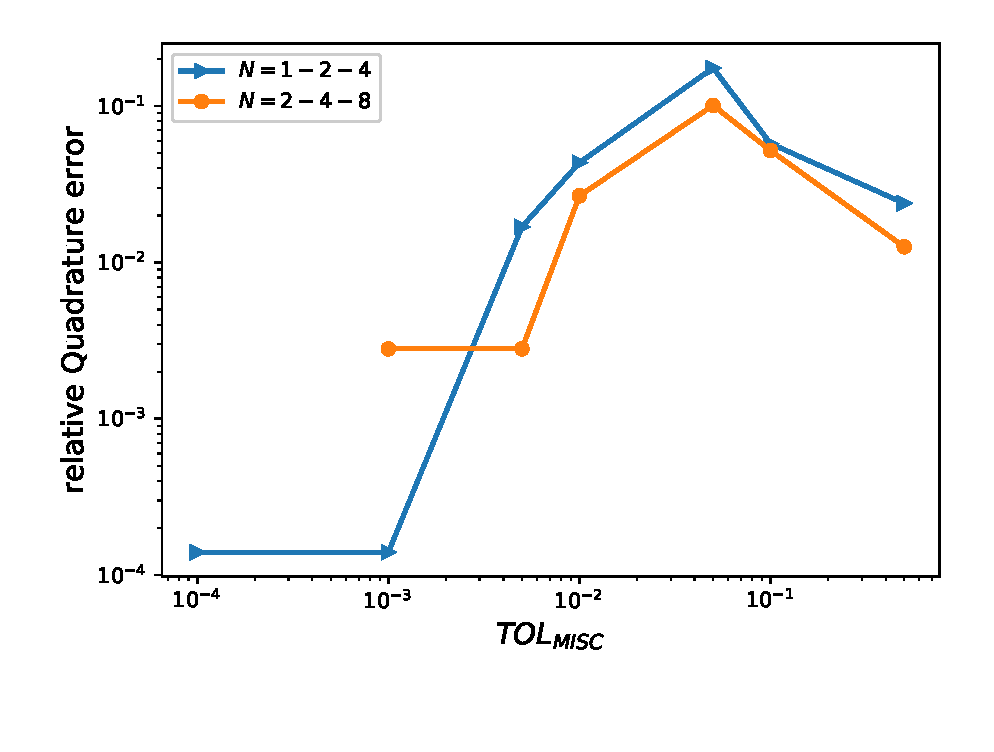
\includegraphics[width=0.35\linewidth]{./figures/rBergomi_MISC_quadratre_error/vs_TOL/set1/relative_quad_error_wrt_MISC_TOL_set1_rich_level2}
%	
%	
%	\caption{Quadrature error of MISC, with different tolerances, to compute call option price of the different tolerances for different number of time steps. Case  set $1$ parameters, with Richardson extrapolation (level $2$).  See detailed values  in table \ref{Quadrature error of MISC to compute Call option price of the different tolerances for different number of time steps. Case set $1$ parameters, with Richardson extrapolation(level $2$). The numbers between parentheses are the corresponding absolute errors.}.}
%	\label{fig:Quadrature_error_set1_rich_level2}
%\end{figure}
%
%
%
%\FloatBarrier
%\begin{table}[!h]
%	\centering
%	\begin{tabular}{l*{6}{c}r}
%		Method \textbackslash  Steps            & $1-2-4$ & $2-4-8$  \\
%		\hline
%%		MISC ($\text{TOL}_{\text{MISC}}=5.10^{-1}$)  & $\mathbf{0.1698
%%		}$ & $\mathbf{ 0.0150}$  \\
%		MISC ($\text{TOL}_{\text{MISC}}=10^{-1}$)  & $\mathbf{0.2035
%		}$ & $\mathbf{ 0.0544}$ \\
%%		MISC ($\text{TOL}_{\text{MISC}}=5.10^{-2}$)  & $\mathbf{0.3214
%%		}$ & $\mathbf{    0.1035}$  \\
%		MISC ($\text{TOL}_{\text{MISC}}=10^{-2}$)  & $\mathbf{0.1894}$ & $\mathbf{  0.0291}$   \\	
%		MISC ($\text{TOL}_{\text{MISC}}=5.10^{-3}$)  & $\mathbf{\red{0.1628}}$ & $\mathbf{\red{0.0052}}$   \\
%%		MISC ($\text{TOL}_{\text{MISC}}=10^{-3}$)  & $\mathbf{0.1460}$ & $\mathbf{0.0052}$   \\
%%		MISC ($\text{TOL}_{\text{MISC}}=10^{-4}$)  & $\mathbf{0.1460}$ & $\mathbf{-}$  \\
%		\hline
%		MC   & $\mathbf{\red{0.1628}}$  & $\mathbf{\red{0.0052}}$    \\
%		\hline
%	\end{tabular}
%	\caption{Total  relative error of MISC, with different tolerances, and MC to compute call option price for different number of time steps. Case set $1$ parameters in table \ref{table:Reference solution, using MC with $500$ time steps, of Call option price under rBergomi model, for different parameter constellation.}, with Richardson extrapolation(level $2$). The values marked in red, for MISC method, correspond to the total relative errors associated with  stable quadrature errors for MISC, and will be used for complexity comparison against MC.}
%	\label{Total  error of MISC and MC to compute Call option price of the different tolerances for different number of time steps. Case set $1$ parameters, with Richardson extrapolation(level $2$). The numbers between parentheses are the corresponding absolute errors.}
%\end{table}
%
%\FloatBarrier
%
%\begin{table}[!h]
%	\centering
%	\begin{tabular}{l*{6}{c}r}
%		Method \textbackslash  Steps            & $1-2-4$ & $2-4-8$   \\
%		\hline
%%		MISC ($\text{TOL}_{\text{MISC}}=5.10^{-1}$)  & $0.2$ & $0.3$  \\
%		MISC ($\text{TOL}_{\text{MISC}}=10^{-1}$)  & $0.25$ & $2$ &   \\
%%		MISC ($\text{TOL}_{\text{MISC}}=5.10^{-2}$)  & $0.55$ & $5$  \\
%		MISC ($\text{TOL}_{\text{MISC}}=10^{-2}$)  & $2$ & $24$   \\
%		MISC ($\text{TOL}_{\text{MISC}}=5.10^{-3}$)  & $\red{5}$ & $\red{64}$  \\	
%%		MISC ($\text{TOL}_{\text{MISC}}=10^{-3}$)  & $24$ & $1067$  \\	
%%		MISC ($\text{TOL}_{\text{MISC}}=10^{-4}$)  & $ 233$ & $-$   \\
%		\hline
%		MC    & $\red{20}$  & $\red{231}$  \\
%		
%		\hline
%		Ratio of $\left(\text{MC}/ \text{MISC} \right)$  &$\red{4}$ & $\red{  3.6}$   \\
%		\hline
%	\end{tabular}
%	\caption{Comparison of the computational time (in Seconds) of  MC and MISC, using Richardson extrapolation (level $2$), used to compute call option price of the rBergomi model for different number of time steps. Case set $1$ parameters in table \ref{table:Reference solution, using MC with $500$ time steps, of Call option price under rBergomi model, for different parameter constellation.}. The
%		average MC CPU time is computed over 10 runs.}
%	\label{Comparsion of the computational time of  MC and MISC, using Richardson extrapolation (level $2$), used to compute Call option price of rBergomi model for different number of time steps. Case set $1$ parameters}
%\end{table}
%
%
%
%\FloatBarrier
%
%
%
%
%
%
%
%\begin{figure}[h!]
%	\centering
%	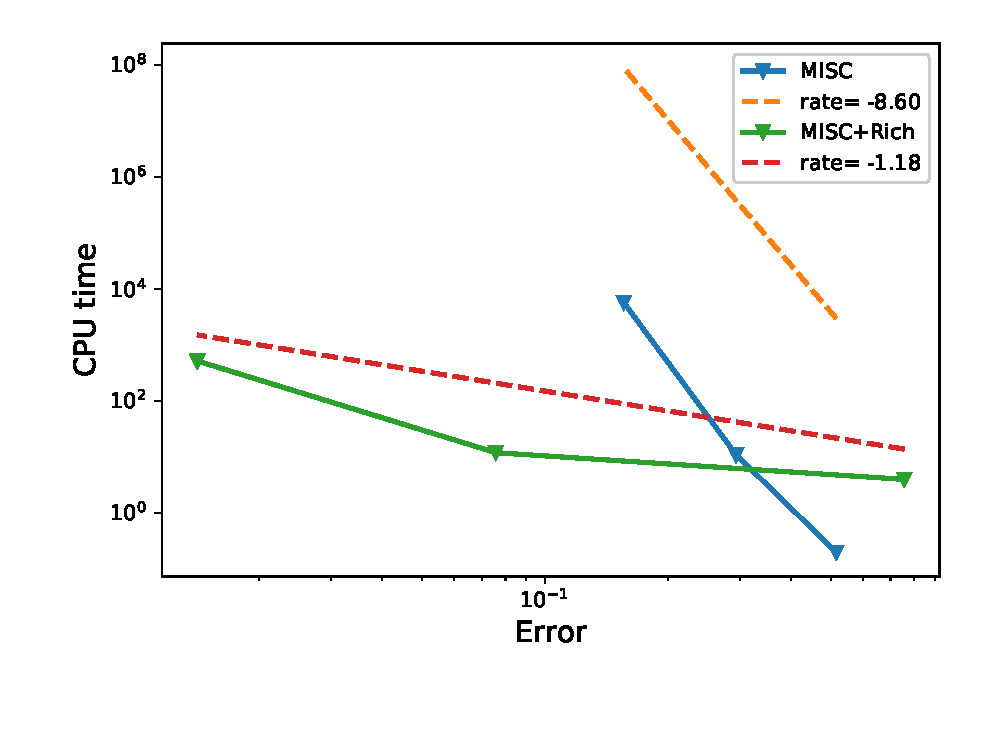
\includegraphics[width=0.35\linewidth]{./figures/rBergomi_Complexity_rates/set1/error_vs_time_set1_comparison}
%	
%	\caption{Complexity plot for  MISC (with and without) Richardson extrapolation for case set $1$ parameters of table \ref{table:Reference solution, using MC with $500$ time steps, of Call option price under rBergomi model, for different parameter constellation.}.}
%	\label{fig:Complexity plot for  MISC for Case set $1$ parameters, comparison}
%\end{figure}
%
%\FloatBarrier
%
%
%


\subsubsection{Case of set $1$ parameters in Table \ref{table:Reference solution, using MC with $500$ time steps, of Call option price under rBergomi model, for different parameter constellation.} }
\label{sec:Case of set $2$ parameters_linear}

For the case of set $1$, we conduct our numerical experiments for $3$ different scenarios: i) without Richardson extrapolation (see Tables \ref{Total error of MISC and MC to compute Call option price of the different tolerances for different number of time steps. Case $K=1$, $H=0.07$, without Richardson extrapolation. The numbers between parentheses are the corresponding absolute errors,linear} and \ref{Comparsion of the computational time of  MC and MISC, used to compute Call option price of rBergomi model for different number of time steps. Case $K=1, H=0.07$, linear}), ii) with (level $1$) Richardson extrapolation (see Tables \ref{Total  error of MISC and MC to compute Call option price of the different tolerances for different number of time steps. Case set $2$ parameters, with Richardson extrapolation(level $1$). The numbers between parentheses are the corresponding absolute errors,relative} and \ref{Comparsion of the computational time of  MC and MISC, using Richardson extrapolation (level $1$), used to compute Call option price of rBergomi model for different number of time steps. Case set $2$ parameters,linear}), and iii) with (level $2$) Richardson extrapolation (see Tables \ref{Total  error of MISC and MC to compute Call option price of the different tolerances for different number of time steps. Case set $2$ parameters, with Richardson extrapolation(level $2$). The numbers between parentheses are the corresponding absolute errors,linear} and \ref{Comparsion of the computational time of  MC and MISC, using Richardson extrapolation (level $2$), used to compute Call option price of rBergomi model for different number of time steps. Case set $2$ parameters,linear}).  Our numerical experiments show that  MISC coupled with (level $1$) Richardson extrapolation is $19$ times faster than MC coupled with (level $1$) Richardson extrapolation, to achieve a total relative error around $8\%$ and $3.5$ times faster than MC, to achieve a total relative error around $2\%$. This gain is improved when applying level $2$ Richardson extrapolation. In fact,  MISC coupled with (level $2$)  Richardson extrapolation is $17$ times faster than MC coupled with (level $2$)  Richardson extrapolation, to achieve a total relative error below  $1\%$. Applying Richardson extrapolation brought a significant improvement for MISC (see Figure \ref{fig:Complexity plot for  MISC for Case set $2$ parameters, comparison} and related tables).

%\subsubsection*{Without Richardson extrapolation}
%\begin{table}[!h]
%	\centering
%	\begin{tabular}{l*{6}{c}r}
%		Method \textbackslash  Steps            & $2$ & $4$ & $8$  \\
%		\hline
%%		MISC ($\text{TOL}_{\text{MISC}}=5.10^{-1}$)  & $0.1097$ & $0.0926$ & $0.0807$  \\
%		MISC ($\text{TOL}_{\text{MISC}}=10^{-1}$)  &$0.1097$ & $0.0926$ & $0.0791$   \\
%%		MISC ($\text{TOL}_{\text{MISC}}=5.10^{-2}$)  & $0.1097$ & $0.0890$ & $0.0849$  \\
%		MISC ($\text{TOL}_{\text{MISC}}=10^{-2}$)  & $0.1119$&  $0.1023$ & $0.0910$  \\
%		MISC ($\text{TOL}_{\text{MISC}}=10^{-3}$)        & $0.1195$ &$0.1023$ &   $0.0910$  \\
%		MISC ($\text{TOL}_{\text{MISC}}=10^{-4}$)        & $0.1218$ &$0.1023$ &  $-$  \\
%		\hline
%		MC method ($M=8.10^{6}$)   & $0.1218 $  & $0.1024 $  & $0.0914$  \\		
%		\hline
%	\end{tabular}
%	\caption{ Call option price of the different methods for different number of time steps. Case of set $2$ parameters in table \ref{table:Reference solution, using MC with $500$ time steps, of Call option price under rBergomi model, for different parameter constellation.}, without Richardson extrapolation.}
%	\label{table: Call option price of the different methods for different number of time steps. Case set 2_linear}
%\end{table}

%We show through table \ref{Bias and Statistical errors of MC ($M=10^6$)  for computing Call option price  for different number of time steps. Case set $2$ parameters, without Richardson extrapolation. The numbers between parentheses are the corresponding absolute errors.} the bias and  the statistical error for MC method, related to Section \ref{sec:Weak error plots_no_change}. 
%\FloatBarrier
%\begin{table}[!h]
%	\centering
%	\begin{tabular}{l*{6}{c}r}
%		Method \textbackslash  Steps            & $2$ & $4$ & $8$   \\
%		\hline
%		MC Bias ($M=8.10^6$)   & $0.54
%		$  & $0.29$  & $0.15$   \\	
%		
%		MC Statistical error ($M=8.10^6$)  & $2.5e-03$  & $1.3e-03$  & $6.3e-04$  \\	
%	
%		\hline
%	\end{tabular}
%	\caption{Relative bias and statistical errors of MC, without Richardson extrapolation,  for computing call option price  for different number of time steps}
%	\label{Bias and Statistical errors of MC ($M=10^6$)  for computing Call option price  for different number of time steps. Case set $2$ parameters, without Richardson extrapolation. The numbers between parentheses are the corresponding absolute errors.}
%\end{table}




%In figure \ref{fig:Quadrature_error_set2_linear}, we plot the behavior of  the relative quadrature error with respect to $\text{TOL}_{\text{MISC}}$. The quadrature error (see \eqref{eq:quadrature error}) is computed by subtracting the MISC solution from the biased solution, computed with sufficiently large  number of samples.



 
%\begin{figure}[h!]
%	\centering
%	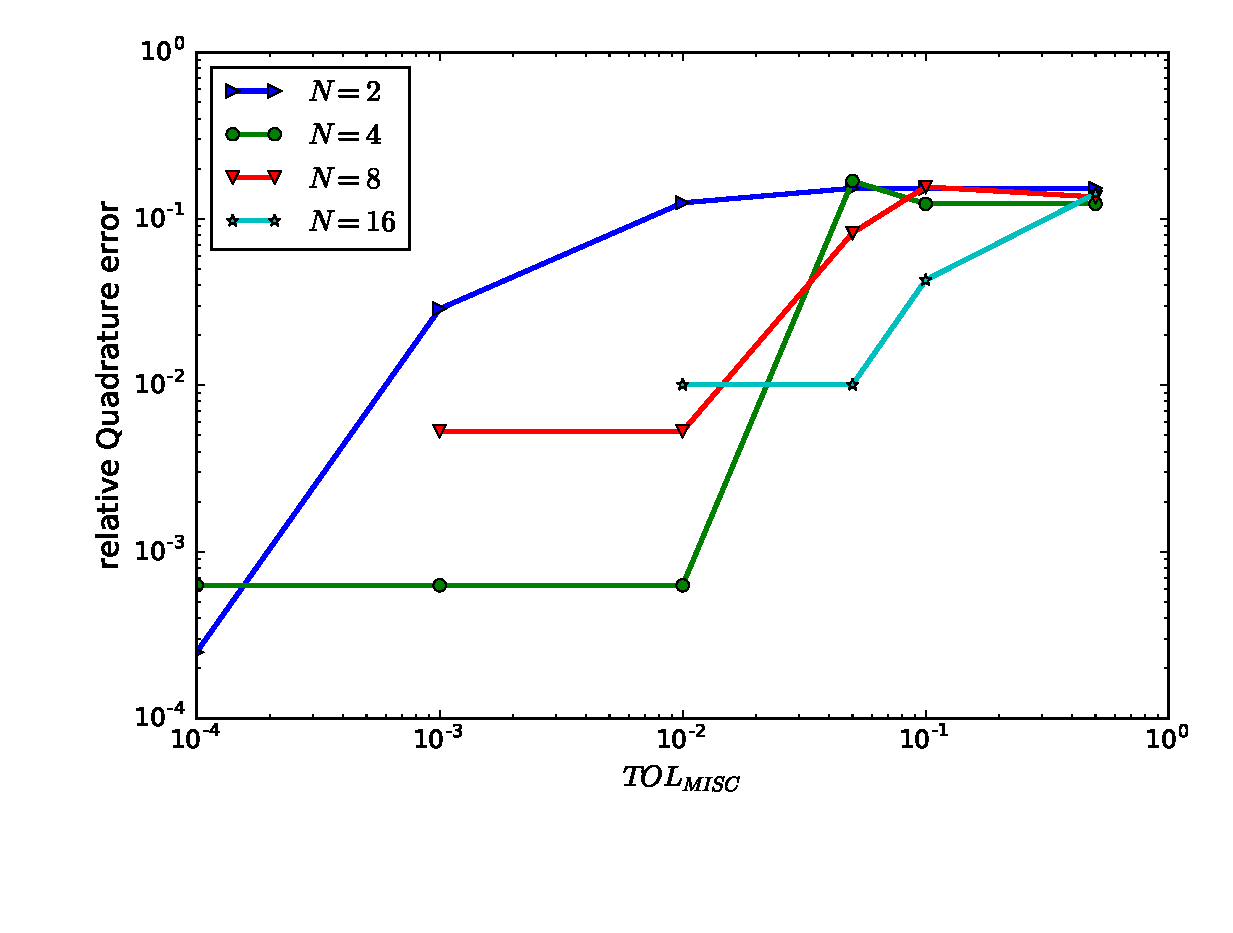
\includegraphics[width=0.4\linewidth]{./figures/rBergomi_MISC_quadratre_error/vs_TOL/set2/relative_quad_error_wrt_MISC_TOL_set2_non_rich_linear}
%	
%	
%	\caption{Quadrature error of MISC, without Richardson extrapolation, with different tolerances, to compute call option price for different number of time steps.}
%%	 See detailed values  in table \ref{Quadrature error of MISC to compute Call option price of the different tolerances for different number of time steps. Case  set $2$ parameters, without Richardson extrapolation. The numbers between parentheses are the corresponding absolute errors,linear}.}
%	\label{fig:Quadrature_error_set2_linear}
%\end{figure}





\FloatBarrier

\begin{table}[h!]
	\centering
	\begin{tabular}{l*{6}{c}r}
		Method \textbackslash  Steps            & $2$ & $4$ & $8$   \\
		\hline

		MISC ($\text{TOL}_{\text{MISC}}=10^{-1}$)  & $\underset{(0.54,0.15)}{\mathbf{
			0.69}}$& $ \underset{(0.29,0.13)}{\mathbf{    
			0.42}}$ & $ \underset{(0.15,0.16)}{\mathbf{     
			0.31
		}}$   \\

		MISC ($\text{TOL}_{\text{MISC}}=10^{-2}$)  & $\underset{(0.54,0.12)}{\mathbf{ 
			0.66}}$ & $ \underset{(0.29,6e-04)}{\mathbf{  \red{ 
				0.29
			}
		}}$ & $\underset{(0.15,0.01)}{\mathbf{ \red{    0.16}}}$   \\
		MISC ($\text{TOL}_{\text{MISC}}=10^{-3}$)        & $\underset{(0.54,0.10)}{\mathbf{
			0.64}}$  &  $ \underset{(0.29,6e-04)}{\mathbf{
			0.29
		}}$ &  $\underset{(0.15,0.01)}{\mathbf{    0.16}}$ \\
		MISC ($\text{TOL}_{\text{MISC}}=10^{-4}$)        & $\underset{(0.54,3e-04)}{\mathbf{       \red{0.54}}}$  & $ \underset{(0.29,6e-04)}{\mathbf{
			0.29
		}}$  &  $-$ \\
		\hline
		MC    & $\underset{(0.54,3e-03)}{\mathbf{0.54}}$  & $\underset{(0.29,1e-03)}{\mathbf{0.29}}$  &$\underset{(0.15,0.01)}{
				\mathbf{0.16}}$  \\	
		M(\# MC samples)   & $8 \times 10^6$  & $8 \times 10^6$  &$10^5$  \\	
		\hline
	\end{tabular}
	\caption{Total relative error of MISC, without Richardson extrapolation, with different tolerances, and MC to compute call option price for different number of time steps. The values marked in red correspond to the total relative errors associated with  asymptotic quadrature errors for MISC, and will be used for computational work comparison against MC. The values between parentheses correspond to the different errors contributing to the total relative error: for MISC we report the bias and quadrature errors and for MC we report the bias and the statistical errors estimates.}
	\label{Total error of MISC and MC to compute Call option price of the different tolerances for different number of time steps. Case $K=1$, $H=0.07$, without Richardson extrapolation. The numbers between parentheses are the corresponding absolute errors,linear}
\end{table}
\FloatBarrier




\begin{table}[htbp]
	\centering
	\begin{tabular}{l*{6}{c}r}
		Method \textbackslash  Steps            & $2$ & $4$ & $8$   \\
		\hline
%		MISC ($\text{TOL}_{\text{MISC}}=5.10^{-1}$)  & $0.08$ & $0.13$ & $0.2$ \\
		MISC ($\text{TOL}_{\text{MISC}}=10^{-1}$)  & $0.08$ & $0.13$ & $0.7$   \\
%		MISC ($\text{TOL}_{\text{MISC}}=5.10^{-2}$)  & $0.08$ & $0.25$ & $7$   \\
		MISC ($\text{TOL}_{\text{MISC}}=10^{-2}$)  & $0.2$& $\red{5}$ & $\red{333}$   \\
		MISC ($\text{TOL}_{\text{MISC}}=10^{-3}$)  &  $2$ & $73$ & $3650$  \\		
		MISC ($\text{TOL}_{\text{MISC}}=10^{-4}$)  & $\red{43}$ & $1240$ & $-$  \\	
	
		\hline
		MC method & $\red{220}$  & $\red{358}$  & $\red{9}$  \\
		\hline	
		Ratio of CPU time  $\left(\text{MC}/ \text{MISC} \right)$  &$\red{5}$ & $\red{   72 
		}$  & $\red {  0.03	}$   \\
		\hline
	\end{tabular}
	\caption{Comparison of the computational time (in Seconds) of  MC and MISC, used to compute call option price of the rBergomi model for different number of time steps. The
		average MC CPU time is computed over $10$ runs.}
	\label{Comparsion of the computational time of  MC and MISC, used to compute Call option price of rBergomi model for different number of time steps. Case $K=1, H=0.07$, linear}
\end{table}
\FloatBarrier
%\subsubsection*{With Richardson extrapolation (level $1$)}

%\begin{table}[!h]
%	\centering
%	\begin{tabular}{l*{6}{c}r}
%		Method \textbackslash  Steps    &$1-2$         & $2-4$ & $4-8$ \\
%		\hline
%%		MISC ($\text{TOL}_{\text{MISC}}=5.10^{-1}$)  &$0.1260$ & $0.0756$ & $0.0687$\\
%		MISC ($\text{TOL}_{\text{MISC}}=10^{-1}$)  &$0.1260$ & $0.0756$ & $0.0702$   \\
%		MISC ($\text{TOL}_{\text{MISC}}=5.10^{-2}$)   &$0.1260$ & $0.0716$ & $0.0796$    \\
%		MISC ($\text{TOL}_{\text{MISC}}=10^{-2}$)  &$0.1456$ & $0.0838$ & $0.0796$  \\	
%		MISC ($\text{TOL}_{\text{MISC}}=10^{-3}$)  &$0.1497$ & $0.0838$ & $-$ \\
%		
%%		MISC ($\text{TOL}_{\text{MISC}}=10^{-4}$)  &$0.1501$ & $-$ & $-$ \\
%		\hline
%		MC method ($M=10^{6}$)   & $0.1552 $  & $0.0846 $  & $0.0804$  \\		
%		\hline
%	\end{tabular}
%	\caption{Call option price of the different methods for different number of time steps. Case set $2$ parameters of table \ref{table:Reference solution, using MC with $500$ time steps, of Call option price under rBergomi model, for different parameter constellation.}, using Richardson extrapolation (level $1$)}
%	\label{table:  Call option price of the different methods for different number of time steps. Case set $2$ parameter, using Richardson extrapolation (level $1$),linear}
%\end{table}

%\FloatBarrier
%
%\begin{table}[h!]
%	\centering
%	\begin{tabular}{l*{6}{c}r}
%		Method \textbackslash  Steps            & $1-2$ & $2-4$ & $4-8$  \\
%		\hline
%		MC Bias ($M=10^6$)  &$0.96$  & $0.07$  & $0.015$   \\	
%		
%		MC Statistical error ($M=10^6$)   & $1.3e-02$  & $4.1e-03$  & $2.1e-03$  \\	
%		\hline
%	\end{tabular}
%	\caption{Relative bias and statistical errors of MC, with Richardson extrapolation (level $1$), for computing call option price  for different number of time steps. The numbers between parentheses are the corresponding absolute errors.}
%	\label{Bias and Statistical errors of MC ($M=10^6$)  for computing Call option price  for different number of time steps. Case set $2$ parameters, with Richardson extrapolation (level1). The numbers between parentheses are the corresponding absolute errors.}
%\end{table}
%
%
%\FloatBarrier
%
%
%
%
%
%\begin{figure}[h!]
%	\centering
%	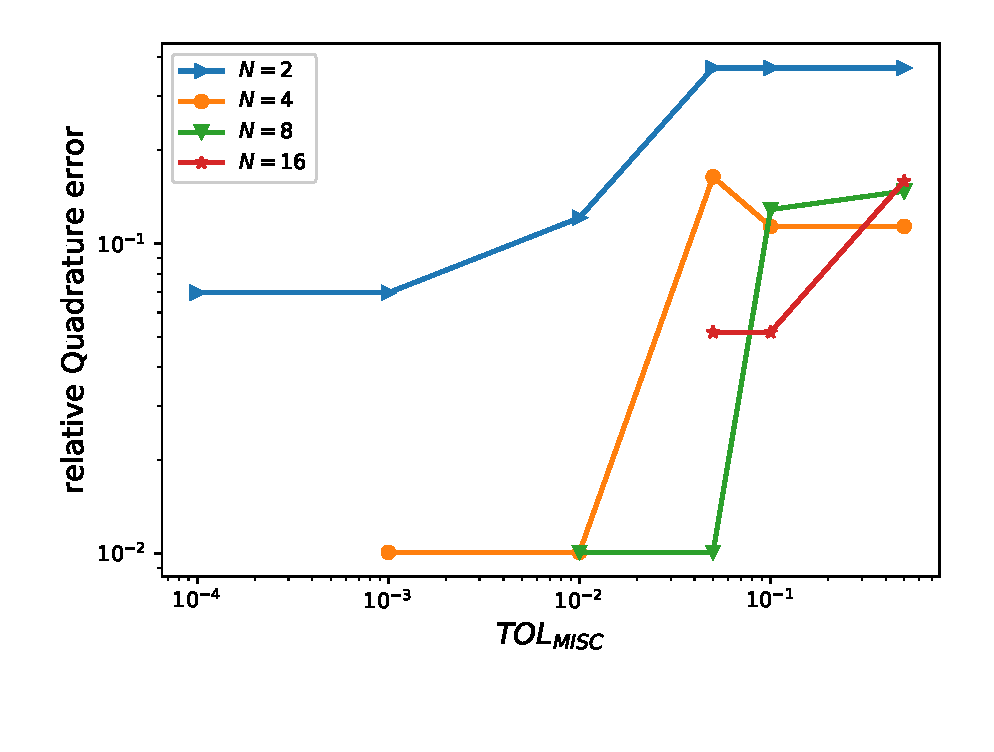
\includegraphics[width=0.4\linewidth]{./figures/rBergomi_MISC_quadratre_error/vs_TOL/set2/relative_quad_error_wrt_MISC_TOL_set2_with_rich_linear}
%	
%	
%	\caption{Quadrature error of MISC,with Richardson extrapolation (level $1$), with different tolerances,  to compute call option price for different number of time steps.}
	
%	  See detailed values  in table \ref{Quadrature error of MISC to compute Call option price of the different tolerances for different number of time steps. Case set $2$ parameters, with Richardson extrapolation(level $1$). The numbers between parentheses are the corresponding absolute errors,linear}.}
%	\label{fig:Quadrature_error_set2_linear_rich}
%\end{figure}


\begin{table}[h!]
	\centering
	\begin{tabular}{l*{6}{c}r}
		Method \textbackslash  Steps            & $1-2$ & $2-4$ & $4-8$  \\
		\hline
		MISC ($\text{TOL}_{\text{MISC}}=10^{-1}$)  & $\underset{(0.96,0.37)}{\mathbf{  1.33}}$ & $\underset{(0.07,0.11)}{\mathbf{0.18}}$ & $\underset{(0.015,0.129)}{\mathbf{0.144}}$   \\
		MISC ($\text{TOL}_{\text{MISC}}=5.10^{-2}$)  & $\underset{(0.96,0.37)}{\mathbf{  1.33}}$ & $\underset{(0.07,0.16)}{\mathbf{ 0.23}}$ & $\underset{(0.015,0.010)}{\mathbf{  \red{0.025}}}$   \\
		MISC ($\text{TOL}_{\text{MISC}}=10^{-2}$)  & $\underset{(0.96,0.12)}{\mathbf{   1.08
		}}$ & $\underset{(0.07,0.01)}{\mathbf{    \red{0.08}}}$ & $\underset{(0.015,0.010)}{\mathbf{ 0.025}}$  \\
		MISC ($\text{TOL}_{\text{MISC}}=10^{-3}$)  & $\underset{(0.96,0.07)}{\mathbf{ \red{  1.03}}}$ & $\underset{(0.07,0.01)}{\mathbf{    0.08}}$ & $\mathbf{-}$  \\
		

		\hline
		
		MC &$\underset{(0.96,0.07)}{\mathbf{1.03}}$  & $\underset{(0.07,0.01)}{\mathbf{0.08}}$ & $\underset{(0.015,0.010)}{\mathbf{0.025}}$  \\
		M(\# MC samples) & $3 \times 10^4$  & $2 \times 10^5$ & $4 \times 10^4$  \\

		\hline
	\end{tabular}
	\caption{Total relative error of MISC, coupled with Richardson extrapolation (level $1$), with different tolerances,  and MC, coupled with Richardson extrapolation (level $1$), to compute call option price  for different number of time steps. The values marked in red correspond to the total relative errors associated with  asymptotic quadrature errors for MISC, and will be used for computational work comparison against MC. The values between parentheses correspond to the different errors contributing to the total relative error: for MISC we report the bias and quadrature errors and for MC we report the bias and the statistical errors.}
	\label{Total  error of MISC and MC to compute Call option price of the different tolerances for different number of time steps. Case set $2$ parameters, with Richardson extrapolation(level $1$). The numbers between parentheses are the corresponding absolute errors,relative}
\end{table}
\FloatBarrier


\begin{table}[h!]
	\centering
	\begin{tabular}{l*{6}{c}r}
		Method \textbackslash  Steps            & $1-2$ & $2-4$ & $4-8$   \\
		\hline
%		MISC ($\text{TOL}_{\text{MISC}}=5.10^{-1}$)  & $0.1$ & $0.18$ & $0.3$   \\
		MISC ($\text{TOL}_{\text{MISC}}=10^{-1}$)  & $0.1$ & $0.18$ & $1.6$  \\
		MISC ($\text{TOL}_{\text{MISC}}=5.10^{-2}$)  & $0.1$ & $0.6$ & $\red{37}$  \\
		MISC ($\text{TOL}_{\text{MISC}}=10^{-2}$)  & $1.3$ & $\red{6}$ & $2382$  \\
		MISC ($\text{TOL}_{\text{MISC}}=10^{-3}$)  & $\red{3.5}$ & $ 244$ & $-$   \\
		
%		MISC ($\text{TOL}_{\text{MISC}}=10^{-4}$)  & $140$ & $-$ & $-$ \\
		\hline	
		MC  &$\red{12}$ & $\red{113}$  & $\red{130}$   \\
		
		\hline	
		Ratio of CPU time $\left(\text{MC}/ \text{MISC} \right)$  &$\red{ 3.4
		}$ & $\red{     18.8
		}$  & $\red{ 3.5}
		$  \\
		\hline
		\end{tabular}
		\caption{Comparison of the computational time (in Seconds) of  MC and MISC, using Richardson extrapolation (level $1$), used to compute call option price of the rBergomi model for different number of time steps. The
			average MC CPU time is computed over $10$ runs.}
		\label{Comparsion of the computational time of  MC and MISC, using Richardson extrapolation (level $1$), used to compute Call option price of rBergomi model for different number of time steps. Case set $2$ parameters,linear}
		\end{table}
		
		\FloatBarrier
%	\subsubsection*{With Richardson extrapolation (level $2$)}
		
%
%		\begin{table}[h!]
%		\centering
%		\begin{tabular}{l*{6}{c}r}
%		Method \textbackslash  Steps           &$1-2-4$ & $2-4-8$ \\
%		\hline
%%		MISC ($\text{TOL}_{\text{MISC}}=5.10^{-1}$)& $0.0587$  & $0.0664 $ \\
%		
%		MISC ($\text{TOL}_{\text{MISC}}=10^{-1}$)  &$0.0587$  &$ 0.0702$   \\
%		MISC ($\text{TOL}_{\text{MISC}}=5.10^{-2}$)  & $0.0401$ & $0.0790$  \\
%		MISC ($\text{TOL}_{\text{MISC}}=10^{-2}$)  & $0.0623$ &  $0.0784$   \\
%%		MISC ($\text{TOL}_{\text{MISC}}=5.10^{-3}$)  & $0.0623$ & $-$   \\
%%		MISC ($\text{TOL}_{\text{MISC}}=10^{-3}$)  & $0.0608$ & $$  \\
%		
%		\hline
%		MC ($M=3.10^6$)  & $ 0.0601$ & $ 0.0787$   \\
%		\hline 
%	\end{tabular}
%	\caption{ Call option price of the different methods for different number of time steps. Case set $2$ parameters in tabel \ref{table:Reference solution, using MC with $500$ time steps, of Call option price under rBergomi model, for different parameter constellation.}, using Richardson extrapolation (level 2).}
%	\label{table: Call option price of the different methods for different number of time steps. Case $K=1,H=0.07$, using Richardson extrapolation_level2,linear}
%\end{table}




%\begin{table}[h!]
%	\centering
%	\begin{tabular}{l*{6}{c}r}
%		Method \textbackslash  Steps            & $1-2-4$ & $2-4-8$  \\
%		\hline
%		MC  Bias  ($M=3.10^6$)   &$ 0.24$  & $ 0.0058$   \\	
%		
%		MC Statistical error ($M=3.10^6$)   & $3.5e-03$  & $  1.8e-03$  \\	
%		
%		
%		
%		\hline
%	\end{tabular}
%	\caption{Relative bias and statistical errors of MC,  with Richardson extrapolation (level $2$), for computing call option price  for different number of time steps. The numbers between parentheses are the corresponding absolute errors.}
%	\label{Bias and Statistical errors of MC ($M=3.10^6$)  for computing Call option price  for different number of time steps. Case set $2$ parameters, with Richardson extrapolation (level2). The numbers between parentheses are the corresponding absolute errors.}
%\end{table}





\begin{table}[!h]
	\centering
	\begin{tabular}{l*{6}{c}r}
		Method \textbackslash  Steps            & $1-2-4$ & $2-4-8$  \\
		\hline

		MISC ($\text{TOL}_{\text{MISC}}=10^{-1}$)  & $\underset{(0.24,0.02)}{\mathbf{ 0.26
		}}$ & $\underset{(0.006,0.107)}{\mathbf{ 0.113}}$ \\
		MISC ($\text{TOL}_{\text{MISC}}=5.10^{-2}$)  & $\underset{(0.24,0.25)}{\mathbf{   0.49
		}}$ & $\underset{(0.006,0.003)}{\mathbf{\red{ 0.009} }}$  \\
		MISC ($\text{TOL}_{\text{MISC}}=10^{-2}$)  & $\underset{(0.24,0.03)}{\mathbf{ \red{0.27}}}$ & $\underset{(0.006,0.003)}{\mathbf{ 0.009 }}$    \\	

		\hline
		MC   & $\underset{(0.24,0.03)}{\mathbf{0.27}}$  & $\underset{(0.006,0.003)}{\mathbf{0.009}}$    \\
			M(\# MC samples) & $5 \times 10^4$  & $7 \times 10^5$   \\
		\hline
	\end{tabular}
	\caption{Total relative  error of MISC, coupled with Richardson extrapolation (level $2$), with different tolerances, and MC, coupled with Richardson extrapolation (level $2$), to compute call option price for different number of time steps. The values marked in red correspond to the total relative errors associated with  asymptotic quadrature errors for MISC, and will be used for computational work comparison against MC. The values between parentheses correspond to the different errors contributing to the total relative error: for MISC we report the bias and quadrature errors and for MC we report the bias and the statistical errors. }
	\label{Total  error of MISC and MC to compute Call option price of the different tolerances for different number of time steps. Case set $2$ parameters, with Richardson extrapolation(level $2$). The numbers between parentheses are the corresponding absolute errors,linear}
\end{table}
\FloatBarrier

\begin{table}[!h]
	\centering
	\begin{tabular}{l*{6}{c}r}
		Method \textbackslash  Steps            & $1-2-4$ & $2-4-8$   \\
		\hline

		MISC ($\text{TOL}_{\text{MISC}}=10^{-1}$)  & $0.2$ & $2$ &   \\
		MISC ($\text{TOL}_{\text{MISC}}=5.10^{-2}$)  & $0.5$ & $\red{74}$  \\
		MISC ($\text{TOL}_{\text{MISC}}=10^{-2}$)  & $\red{9}$ & $3455$   \\
%		MISC ($\text{TOL}_{\text{MISC}}=5.10^{-3}$)  & $30$ & $-$  \\	
%		MISC ($\text{TOL}_{\text{MISC}}=10^{-3}$)  & $693$ & $-$  \\	
		\hline
		MC    & $ \red{  118}$  & $\red{1274}$  \\
		
		\hline
		Ratio of CPU time $\left(\text{MC}/ \text{MISC} \right)$  &$\red{13}$ & $\red{  17}$   \\
		\hline
	\end{tabular}
	\caption{Comparison of the computational time (in Seconds) of  MC and MISC, using Richardson extrapolation (level $2$), used to compute call option price of the rBergomi model for different number of time steps. The
		average MC CPU time is computed over $10$ runs.}
	\label{Comparsion of the computational time of  MC and MISC, using Richardson extrapolation (level $2$), used to compute Call option price of rBergomi model for different number of time steps. Case set $2$ parameters,linear}
\end{table}

\FloatBarrier

\begin{figure}[h!]
	\centering
	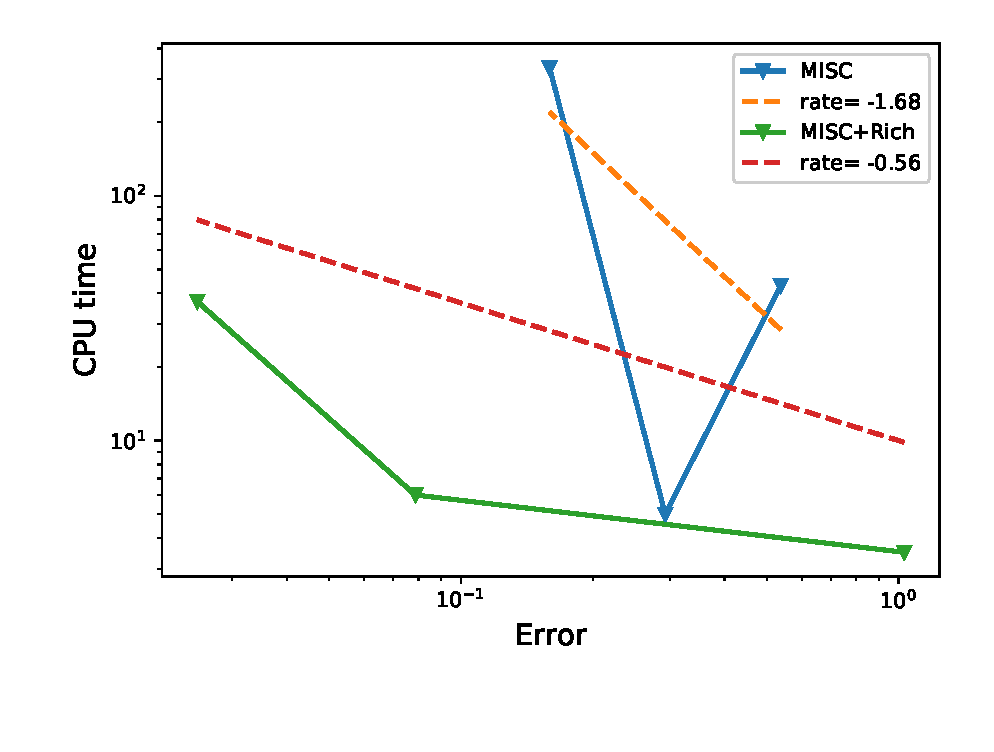
\includegraphics[width=0.5\linewidth]{./figures/rBergomi_Complexity_rates/set2/error_vs_time_set2_comparison_linear}
	
	\caption{Computational work comparison for  MISC (with and without) Richardson extrapolation.}
	\label{fig:Complexity plot for  MISC for Case set $2$ parameters, comparison}
\end{figure}




\FloatBarrier

\subsubsection{Case of set $2$ parameters in Table \ref{table:Reference solution, using MC with $500$ time steps, of Call option price under rBergomi model, for different parameter constellation.}}\label{sec:Case of set 3 parameters}

For the case of set $2$, we conduct our numerical experiments for $2$ different scenarios: i) without Richardson extrapolation (see Figure \ref{fig:Complexity plot for MC and MISC for Case set $3$ parameters} and Tables \ref{Comparsion of the computational time of  MC and MISC, used to compute Call option price of rBergomi model for different number of time steps. Case set3} and \ref{Total error of MISC and MC to compute Call option price of the different tolerances for different number of time steps. Case set 3, without Richardson extrapolation. The numbers between parentheses are the corresponding absolute errors.}), and  ii) with (level $1$) Richardson extrapolation  (see Figure \ref{fig:Complexity plot for  MISC for case set $3$ parameters, comparison} and Tables \ref{Total  error of MISC and MC to compute Call option price of the different tolerances for different number of time steps. Case set $3$ parameters, with Richardson extrapolation(level $1$). The numbers between parentheses are the corresponding absolute errors.} and \ref{Comparsion of the computational time of  MC and MISC, using Richardson extrapolation (level $1$), used to compute Call option price of rBergomi model for different number of time steps. Case set $3$ parameters}). Our numerical experiments show that MISC is  $43$ times faster than MC, to achieve  a total relative error below $1\%$ and $8$ times faster than MC, to achieve a total relative error around $0.1\%$. Using Richardson extrapolation brought an improvement in terms of the  computational work constant compared to using simple MISC.

%\subsubsection*{Without Richardson extrapolation}

%\begin{table}[h!]
%	\centering
%	\begin{tabular}{l*{6}{c}r}
%		Method \textbackslash  Steps            & $2$ & $4$ & $8$ & $16$ &   \\
%		\hline
%%		MISC ($\text{TOL}_{\text{MISC}}=5.10^{-1}$)  & $0.1258$ & $0.1239$ & $0.1231$ & $0.1227$  \\
%		MISC ($\text{TOL}_{\text{MISC}}=10^{-1}$)  & $0.1258$ & $0.1239$ & $0.1231$ & $0.1229$  \\
%%		MISC ($\text{TOL}_{\text{MISC}}=5.10^{-2}$)  & $0.1258$ & $0.1239$ & $0.1231$ & $0.1241$  \\
%		MISC ($\text{TOL}_{\text{MISC}}=10^{-2}$)  & $0.1258$ & $0.1246$ & $0.1248$ & $0.1250$  \\
%		
%		MISC ($\text{TOL}_{\text{MISC}}=10^{-3}$)  & $0.1271$ & $0.1259$ & $0.1252$ & $0.1249$  \\
%		MISC ($\text{TOL}_{\text{MISC}}=10^{-4}$)  & $0.1270$ & $0.1258$ & $0.1252$ & $-$  \\
%		
%%			MISC ($\text{TOL}_{\text{MISC}}=10^{-5}$)  & $0.1270$ &$0.1258$ &  $0.1252$ & $-$  \\
%		\hline
%		MC method ($M=3.10^{6}$)   & $    0.1269$ & $0.1257$  & $0.1253$ & $0.1249$ \\		
%		
%		\hline
%	\end{tabular}
%	\caption{ Call option price of the different methods for different number of time steps. Case of set $3$ parameters in table \ref{table:Reference solution, using MC with $500$ time steps, of Call option price under rBergomi model, for different parameter constellation.}, without Richardson extrapolation.}
%	\label{table: Call option price of the different methods for different number of time steps. Case set 3}
%\end{table}

%\FloatBarrier
%
%\begin{table}[h!]
%	\centering
%	\begin{tabular}{l*{6}{c}r}
%		Method \textbackslash  Steps            & $2$ & $4$ & $8$ & $16$  \\
%		\hline
%		MC Bias ($M=3.10^6$)   & 	$ \underset{(    0.0022)}{\mathbf{0.0174}}$  & $\underset{(0.001)}{\mathbf{0.0078}}$  & $\underset{(0.0005)}{\mathbf{0.0042}}$ & $\underset{(0.0001)}{\mathbf{0.0008}}$\\ 
%		
%		MC Statistical error ($M=3.10^6$)  &  $\underset{(   6.2e-05)} {\mathbf{5.0e-04}}$  & $\underset{(5.9e-05)} {\mathbf{4.7e-04}}$  & $\underset{(5.8e-05)} {\mathbf{4.6e-04 }}$ & $\underset{(5.8e-05)} {\mathbf{4.6e-04 }}$	\\
%		
%		\hline
%	\end{tabular}
%	\caption{Bias and statistical errors of MC   for computing call option price  for different number of time steps. Case set $2$, without Richardson extrapolation. The numbers between parentheses are the corresponding absolute errors.}
%	\label{Bias and Statistical errors of MC ($M=10^6$)  for computing Call option price  for different number of time steps. Case set 3, without Richardson extrapolation. The numbers between parentheses are the corresponding absolute errors.}
%\end{table}
%
%
%
%
%\FloatBarrier
%
%	\begin{figure}[h!]
%		\centering
%		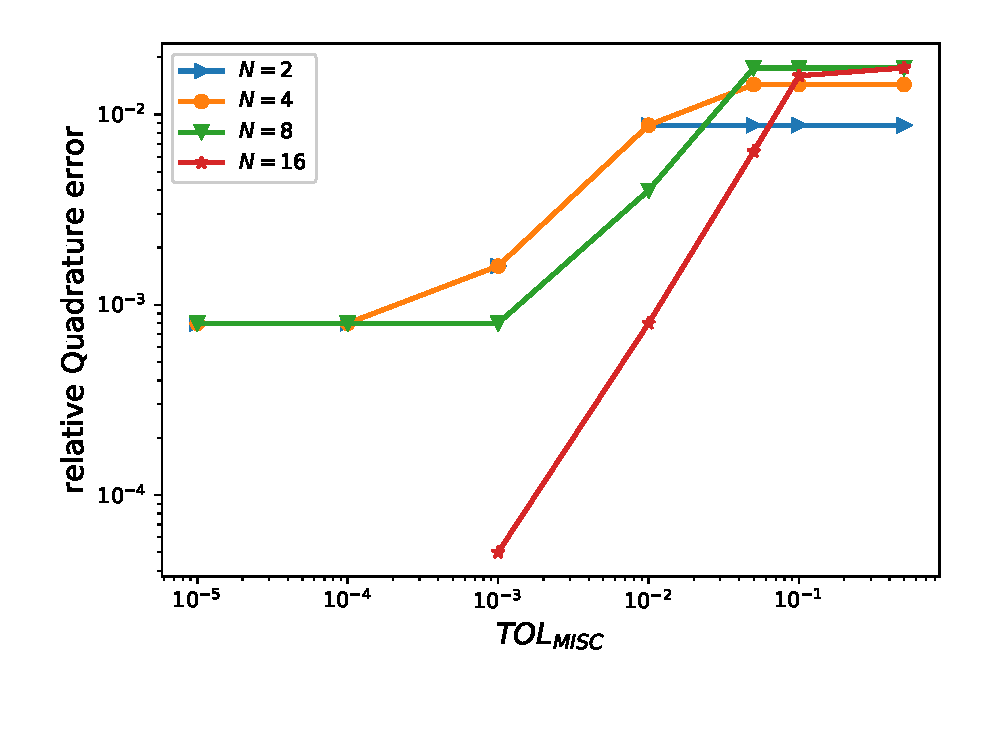
\includegraphics[width=0.35\linewidth]{./figures/rBergomi_MISC_quadratre_error/vs_TOL/set5/relative_quad_error_wrt_MISC_TOL_set5_non_rich}
%	
%	
%	\caption{Quadrature error of MISC, with different tolerances, to compute call option price  for different number of time steps. Case  set $2$ parameters, without Richardson extrapolation. }
%%	 See detailed values  in table \ref{Quadrature error of MISC to compute Call option price of the different tolerances for different number of time steps. Case  set $3$ parameters, without Richardson extrapolation. The numbers between parentheses are the corresponding absolute errors.}.}
%	\label{fig:Quadrature_error_set3}
%\end{figure}
%
\FloatBarrier




\begin{table}[h!]
	\centering
	\begin{tabular}{l*{6}{c}r}
		Method \textbackslash  Steps            & $2$ & $4$ & $8$ & $16$  \\
		\hline

		MISC ($\text{TOL}_{\text{MISC}}=10^{-1}$)  &  $\underset{(0.02,0.01)}{\mathbf{0.03}}$ & $\underset{(0.008,0.014)}{\mathbf{0.022}}$& $\underset{(0.004,0.018)}{\mathbf{ 0.022}}$ & $\underset{(0.001,0.016)}{\mathbf{ 0.017}}$   \\

		MISC ($\text{TOL}_{\text{MISC}}=10^{-2}$)  &  $\underset{(0.02,0.01)}{\mathbf{0.03}}$ & $\underset{(0.008,0.009)}{\mathbf{0.017}}$& $\underset{(0.004,0.004)}{\mathbf{ 0.008}}$ & $\underset{(0.001,4e-04)}{\mathbf{ \red{0.001}}}$  \\
		MISC ($\text{TOL}_{\text{MISC}}=10^{-3}$)  &  $\underset{(0.02,8e-04)}{\mathbf{\red{0.02}}}$ & $\underset{(0.008,8e-04)}{\red{\mathbf{0.009}}}$& $\underset{(0.004,8e-04)}{\mathbf{\red{0.005}}}$  & $\underset{(0.001,4e-04)}{\mathbf{ 0.001}}$  \\
%		MISC ($\text{TOL}_{\text{MISC}}=10^{-4}$)  &  $\underset{(0.02,8e-04)}{\mathbf{\red{0.02}}}$ & $\underset{(0.008,8e-04)}{\mathbf{\red{0.009}}}$& $\underset{(0.004,8e-04)}{\mathbf{0.005}}$ & $\mathbf{ -}$ \\

		\hline
		MC    & $\underset{(0.02,5e-04)}{\mathbf{0.02}}$  &  $\underset{(0.008,5e-04)}{\mathbf{0.009}}$  & $\underset{(0.004,5e-04)}{\mathbf{0.005}}$ & $\underset{(0.001,4e-04)}{\mathbf{0.001}}$  \\	
			M(\# MC samples) 	& $5 \times 10^6$  &  $5 \times 10^6$  & $5 \times 10^6$ & $5 \times 10^6$  \\
		\hline
	\end{tabular}
	\caption{Total relative error of MISC, without Richardson extrapolation,  with different tolerances, and MC to compute call option price for different number of time steps.}
	\label{Total error of MISC and MC to compute Call option price of the different tolerances for different number of time steps. Case set 3, without Richardson extrapolation. The numbers between parentheses are the corresponding absolute errors.}
\end{table}


\FloatBarrier
\begin{table}[h!]
	\centering
	\begin{tabular}{l*{6}{c}r}
		Method \textbackslash  Steps            & $2$ & $4$ & $8$ & $16$ &   \\
		\hline
%		MISC ($\text{TOL}_{\text{MISC}}=5.10^{-1}$)  & $0.1$ & $0.1$ & $0.2$ & $0.4$  \\
		MISC ($\text{TOL}_{\text{MISC}}=10^{-1}$)  & $0.1$ & $0.1$ & $0.2$ & $0.8$ \\
%		MISC ($\text{TOL}_{\text{MISC}}=5.10^{-2}$)  & $0.1$ & $0.1$ & $0.2$ & $22$  \\
		MISC ($\text{TOL}_{\text{MISC}}=10^{-2}$)  & $0.1$ & $0.5$ & $8$ & $\red{92}$ \\
		MISC ($\text{TOL}_{\text{MISC}}=10^{-3}$)  & $\red{0.5}$ & $\red{3}$ & $\red{24}$ & $2226$ \\
%		MISC ($\text{TOL}_{\text{MISC}}=10^{-4}$)  & $\red{1}$ & $\red{6}$ & $80$ & $-$\\
%		MISC ($\text{TOL}_{\text{MISC}}=10^{-5}$)  & $2$ & $32$ & $1760$ & $-$
%		 \\
		\hline
		MC method   & $ \red{122}
		
		$  & $  \red{260}$  & $  \red{427}$ & $ \red{766}
		$  \\	
		\hline
		Ratio of CPU time  $\left(MC/MISC \right)$ & $ \red{244}
		
		$  & $  \red{86}$  & $  \red{  18
		}$ & $ \red{ 8}
		$  \\	
		
		\hline
	\end{tabular}
	\caption{Comparison of the computational time (in Seconds) of  MC and MISC, used to compute call option price of the rBergomi model for different number of time steps. The average  MC CPU time is computed over $10$ runs. }
	\label{Comparsion of the computational time of  MC and MISC, used to compute Call option price of rBergomi model for different number of time steps. Case set3}
\end{table}
\FloatBarrier
	\begin{figure}[h!]
	\centering
	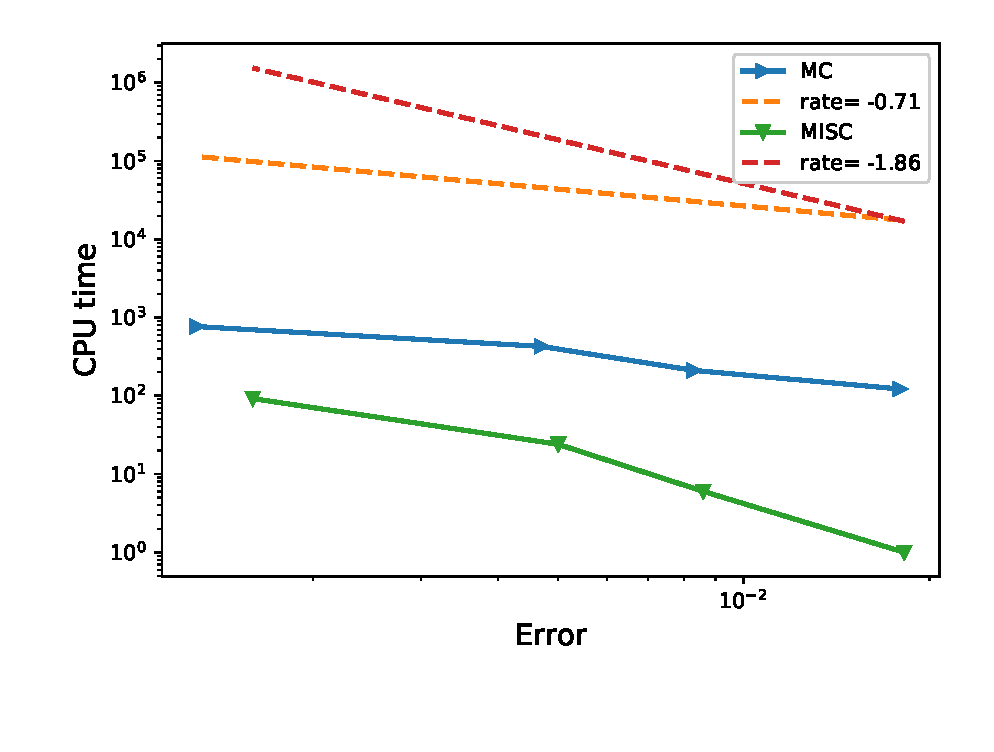
\includegraphics[width=0.5\linewidth]{./figures/rBergomi_Complexity_rates/set5/error_vs_time_set5}

	\caption{Comparison of computational work  for MC and MISC, without Richardson extrapolation.}
	\label{fig:Complexity plot for MC and MISC for Case set $3$ parameters}
\end{figure}



\FloatBarrier

%\subsubsection*{With Richardson extrapolation (level $1$)}
%\FloatBarrier
%\begin{table}[h!]
%	\centering
%	\begin{tabular}{l*{6}{c}r}
%		Method \textbackslash  Steps    &$1-2$         & $2-4$ & $4-8$ & $8-16$\\
%		\hline
%%		MISC ($\text{TOL}_{\text{MISC}}=5.10^{-1}$)   &$ 0.1261$ & $0.1220$ & $0.1222$ & $0.1223$\\
%		MISC ($\text{TOL}_{\text{MISC}}=10^{-1}$)   &$ 0.1261$ & $0.1220$  &$0.1222$ & $0.1226$\\
%%		MISC ($\text{TOL}_{\text{MISC}}=5.10^{-2}$)   &$ 0.1261$ & $0.1220$  & $0.1222$ & $0.1240$ \\
%		MISC ($\text{TOL}_{\text{MISC}}=10^{-2}$)   &$ 0.1267$ & $0.1230$ & $0.1245$ & $0.1247$  \\	
%		MISC ($\text{TOL}_{\text{MISC}}=10^{-3}$)   &$0.1285$ & $0.1247$ & $0.1247$ &  $0.1247$ \\
%%		MISC ($\text{TOL}_{\text{MISC}}=10^{-4}$)  &$0.1285$ & $0.1247$ & $0.1247$ & $-$ \\
%%			MISC ($\text{TOL}_{\text{MISC}}=10^{-5}$)  &$0.1285$ & $0.1247$ &  $0.1247$ & $-$ \\
%	
%		\hline
%		MC method ($M=10^{7}$)   & $     0.1284$  & $ 
%		0.1251$  & $0.1249$ & $  0.1248$ \\		
%		\hline
%	\end{tabular}
%	\caption{Call option price of the different methods for different number of time steps. Case set $3$ parameters of table \ref{table:Reference solution, using MC with $500$ time steps, of Call option price under rBergomi model, for different parameter constellation.}, using Richardson extrapolation (level $1$).}
%	\label{table:  Call option price of the different methods for different number of time steps. Case set $5$ parameter, using Richardson extrapolation (level $3$)}
%\end{table}
%\FloatBarrier
%
%
%\begin{table}[h!]
%	\centering
%	\begin{tabular}{l*{6}{c}r}
%		Method \textbackslash  Steps            & $1-2$ & $2-4$ & $4-8$ & $8-16$  \\
%		\hline
%		MC Bias ($M=10^7$)  &$\underset{(  0.0037
%			)}{\mathbf{0.0295}}$  & $\underset{( 0.0003)}{\mathbf{0.0025}}$  & $\underset{(   0.0001)}{\mathbf{0.0009}}$  & $\underset{(  6.2e-05)}{\mathbf{0.0005}}$ \\	
%		
%		MC Statistical error ($M=10^7$)   & $\underset{(  4.4e-05)}{\mathbf{3.5e-04}}$  & $\underset{(   4.2e-05)}{\mathbf{3.4e-04}}$  & $\underset{(  4.1e-05)}{\mathbf{3.3e-04}}$ & $\underset{(  4.1e-05)}{\mathbf{3.3e-04}}$ \\	
%	
%		\hline
%	\end{tabular}
%	\caption{Bias and statistical errors of MC   for computing call option price  for different number of time steps. Case set $2$ parameters in table \ref{table:Reference solution, using MC with $500$ time steps, of Call option price under rBergomi model, for different parameter constellation.}, with Richardson extrapolation (level $1$). The numbers between parentheses are the corresponding absolute errors.}
%	\label{Bias and Statistical errors of MC ($M=10^7$)  for computing Call option price  for different number of time steps. Case set $3$ parameters, with Richardson extrapolation (level1). The numbers between parentheses are the corresponding absolute errors.}
%\end{table}
%
%
%
%\FloatBarrier
%
%
%
%
%\begin{figure}[h!]
%	\centering
%	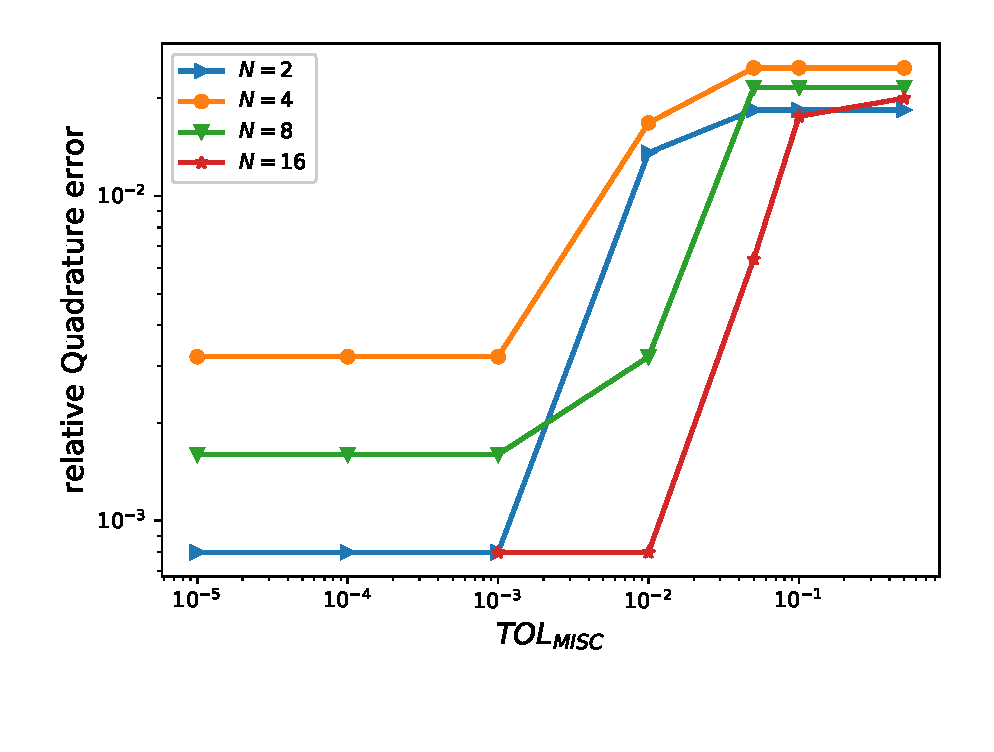
\includegraphics[width=0.35\linewidth]{./figures/rBergomi_MISC_quadratre_error/vs_TOL/set5/relative_quad_error_wrt_MISC_TOL_set5_with_rich}
%	
%	
%	\caption{Quadrature error of MISC, with  different tolerances,  to compute call option price, for different number of time steps. Case  set $2$ parameters, with Richardson extrapolation.}
%%	  See detailed values  in table \ref{Quadrature error of MISC to compute Call option price of the different tolerances for different number of time steps. Case set $3$ parameters, with Richardson extrapolation(level $1$). The numbers between parentheses are the corresponding absolute errors.}.}
%	\label{fig:Quadrature_error_set3_rich}
%\end{figure}




\FloatBarrier
\begin{table}[h!]
	\centering
	\begin{tabular}{l*{6}{c}r}
		Method \textbackslash  Steps           & $2-4$ & $4-8$ & $8-16$  \\
		\hline

		MISC ($\text{TOL}_{\text{MISC}}=10^{-1}$)  &$\underset{(0.003,0.024)}{\mathbf{0.027}}$  &$\underset{(0.001,0.022)}{\mathbf{0.023}}$ & $\underset{(0.001,0.017)} {\mathbf{0.018}}$  \\

			MISC ($\text{TOL}_{\text{MISC}}=10^{-2}$)  & $\underset{(0.003,0.016)}{\mathbf{0.019}}$  & $\underset{(0.001,0.003)}{\mathbf{0.004}}$ & $\underset{(0.001,0.001)} {\red{\mathbf{0.002}}}$  \\
		MISC ($\text{TOL}_{\text{MISC}}=10^{-3}$)  & $\underset{(0.003,0.003)}{\red{\mathbf{0.006}}}$  & $\underset{(0.001,0.002)}{\red{\mathbf{0.003}}}$ & $\underset{(0.001,0.001)} {\mathbf{0.002}}$  \\
	
	\hline

		MC    & $\underset{(0.003,0.003)}{\mathbf{0.007}}$  &   $\underset{(0.001,0.002)}{\mathbf{0.003}}$  &  $\underset{(0.001,0.001)}{\mathbf{0.002}}$  \\
			M(\# MC samples) & $5 \times 10^4$  &   $4 \times 10^5$  &  $2 \times 10^6$  \\
		\hline
	\end{tabular}
	\caption{Total relative error of MISC, coupled with Richardson extrapolation (level $1$), with different tolerances, and MC, coupled with Richardson extrapolation (level $1$), to compute call option price  for different number of time steps.}
	\label{Total  error of MISC and MC to compute Call option price of the different tolerances for different number of time steps. Case set $3$ parameters, with Richardson extrapolation(level $1$). The numbers between parentheses are the corresponding absolute errors.}
\end{table}

\FloatBarrier

\begin{table}[h!]
	\centering
	\begin{tabular}{l*{6}{c}r}
		Method \textbackslash  Steps            & $2-4$ & $4-8$ & $8-16$ &   \\
		\hline
%		MISC ($\text{TOL}_{\text{MISC}}=5.10^{-1}$)    & $0.15$ & $0.25$ & $0.5$  \\
		MISC ($\text{TOL}_{\text{MISC}}=10^{-1}$)   & $0.15$ & $0.25$ & $1$  \\
%		MISC ($\text{TOL}_{\text{MISC}}=5.10^{-2}$)    &  $0.15$ & $0.25$ & $12.5$  \\
		MISC ($\text{TOL}_{\text{MISC}}=10^{-2}$)   & $0.6$ & $10$ & $\red{112}$  \\
		MISC ($\text{TOL}_{\text{MISC}}=10^{-3}$)  & $\red{3.5}$ & $\red{34}$ & $3150$ \\
%		MISC ($\text{TOL}_{\text{MISC}}=10^{-4}$) & $11$ & $328$ & $-$  \\
%		MISC ($\text{TOL}_{\text{MISC}}=10^{-5}$)   & $39$ & $2160$ & $-$  \\
		\hline	
			MC  & $\red{45}$  & $\red{438}$  & $\red{2240}$ \\
			
			\hline
				Ratio of CPU time  $\left(\text{MC}/ \text{MISC} \right)$   & $\red{13}$  & $\red{13}$  & $\red{20}$ \\

		\hline
	\end{tabular}
	\caption{Comparison of the computational time (in Seconds) of  MC and MISC, using Richardson extrapolation (level $1$), used to compute call option price of the rBergomi model for different number of time steps. The
average MC CPU time is computed over 10 runs.}
	\label{Comparsion of the computational time of  MC and MISC, using Richardson extrapolation (level $1$), used to compute Call option price of rBergomi model for different number of time steps. Case set $3$ parameters}
\end{table}

\FloatBarrier


	\begin{figure}[h!]
	\centering
	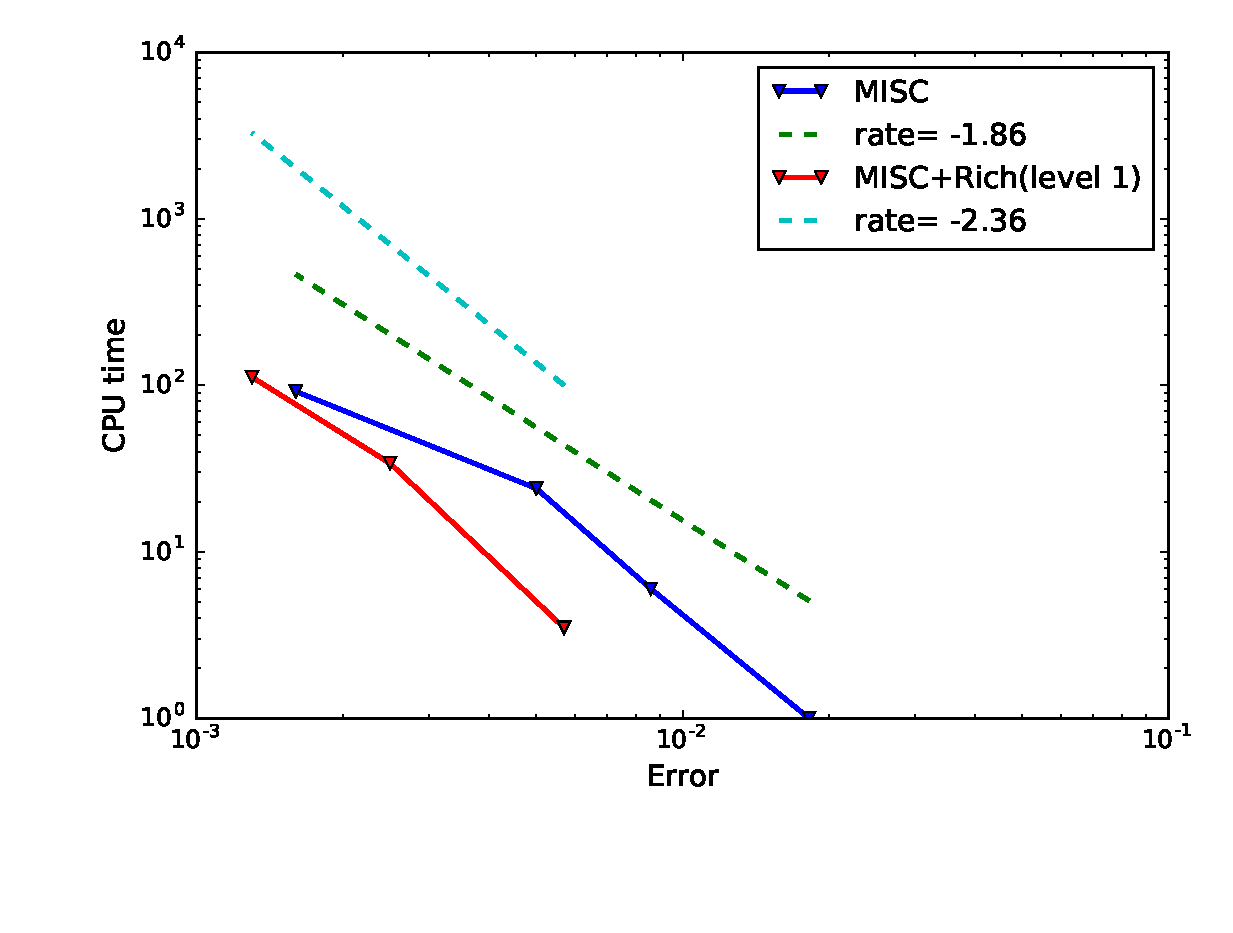
\includegraphics[width=0.5\linewidth]{./figures/rBergomi_Complexity_rates/set5/error_vs_time_set5_comparison}
	
	\caption{Computational work for  MISC (with and without) Richardson extrapolation.}
	\label{fig:Complexity plot for  MISC for case set $3$ parameters, comparison}
\end{figure}


\FloatBarrier
\subsubsection{Case of set $3$ parameters in Table \ref{table:Reference solution, using MC with $500$ time steps, of Call option price under rBergomi model, for different parameter constellation.}}\label{sec:Case of set 4 parameters}


For the case of set $3$, we just conduct our numerical experiments for the case without Richardson extrapolation, since the results show that we meet a small enough error tolerance without the need to apply   Richardson extrapolation.  Our numerical experiments show that MISC is  $141$ times faster than MC, to achieve a total relative error around $0.6\%$ (see Figure \ref{fig:Complexity plot for MC and MISC for case set $4$ parameters} and Tables \ref{Comparsion of the computational time of  MC and MISC, used to compute Call option price of rBergomi model for different number of time steps. Case set4} and \ref{Total error of MISC and MC to compute Call option price of the different tolerances for different number of time steps. Case set 4, without Richardson extrapolation. The numbers between parentheses are the corresponding absolute errors.}).

%\FloatBarrier
%\begin{table}[h!]
%	\centering
%	\begin{tabular}{l*{6}{c}r}
%		Method \textbackslash  Steps            & $2$ & $4$ & $8$ & $16$ &   \\
%		\hline
%%		MISC ($\text{TOL}_{\text{MISC}}=5.10^{-1}$)  & $0.2413$ & $0.2403$ & $0.2403$ & $0.2396$  \\
%		MISC ($\text{TOL}_{\text{MISC}}=10^{-1}$)  & $0.2413$ &$0.2403$& $0.2403$ & $0.2397$   \\
%%		MISC ($\text{TOL}_{\text{MISC}}=5.10^{-2}$)  &$0.2413$ & $0.2403$ & $0.2403$ & $0.2406$  \\
%		MISC ($\text{TOL}_{\text{MISC}}=10^{-2}$)  &$0.2413$ & $0.2403$ & $0.2409$ & $0.2413$  \\
%		
%		MISC ($\text{TOL}_{\text{MISC}}=10^{-3}$)  & $0.2413$ & $0.2411$ & $0.2414$ & $0.2413$  \\
%		MISC ($\text{TOL}_{\text{MISC}}=10^{-4}$)  &  $0.2421$ & $0.2416$ & $0.2414$ & $-$  \\
%		
%%		MISC ($\text{TOL}_{\text{MISC}}=10^{-5}$)  & $0.2421$ &$0.2416$ &  $0.2414$ & $-$  \\
%		\hline
%		MC method ($M=5.10^{6}$)   & $0.2420$ & $0.2416$  & $0.2414$ & $0.2413$ \\		
%		
%		\hline
%	\end{tabular}
%	\caption{ Call option price of the different methods for different number of time steps. Case set $4$ parameters in table \ref{table:Reference solution, using MC with $500$ time steps, of Call option price under rBergomi model, for different parameter constellation.}, without Richardson extrapolation.}
%	\label{table: Call option price of the different methods for different number of time steps. Case set 4}
%\end{table}
%\FloatBarrier
%
%\begin{table}[h!]
%	\centering
%	\begin{tabular}{l*{6}{c}r}
%		Method \textbackslash  Steps            & $2$ & $4$ & $8$ & $16$  \\
%		\hline
%		MC Bias ($M=5.10^6$)   & 	$ \underset{(    0.0013)}{\mathbf{0.0054}}$  & $\underset{(0.0008)}{\mathbf{0.0035
%		}}$  & $\underset{(0.0007)}{\mathbf{0.0029}}$ & $\underset{(0.0006)}{\mathbf{0.0024}}$\\ 
%		
%		MC Statistical error ($M=5.10^6$)  &  $\underset{(   8.3e-05)} {\mathbf{3.4e-04}}$  & $\underset{(8.1e-05)} {\mathbf{3.4e-04}}$  & $\underset{(8.0e-05)} {\mathbf{3.3e-04 }}$ & $\underset{(8.0e-05)} {\mathbf{3.3e-04}}$	\\
%		
%		\hline
%	\end{tabular}
%	\caption{Bias and statistical errors of MC   for computing call option price  for different number of time steps. Case set $3$, without Richardson extrapolation. The numbers between parentheses are the corresponding absolute errors.}
%	\label{Bias and Statistical errors of MC ($M=5.10^6$)  for computing Call option price  for different number of time steps. Case set 4, without Richardson extrapolation. The numbers between parentheses are the corresponding absolute errors.}
%\end{table}
%
%
%\FloatBarrier
%
%
%\begin{figure}[h!]
%	\centering
%	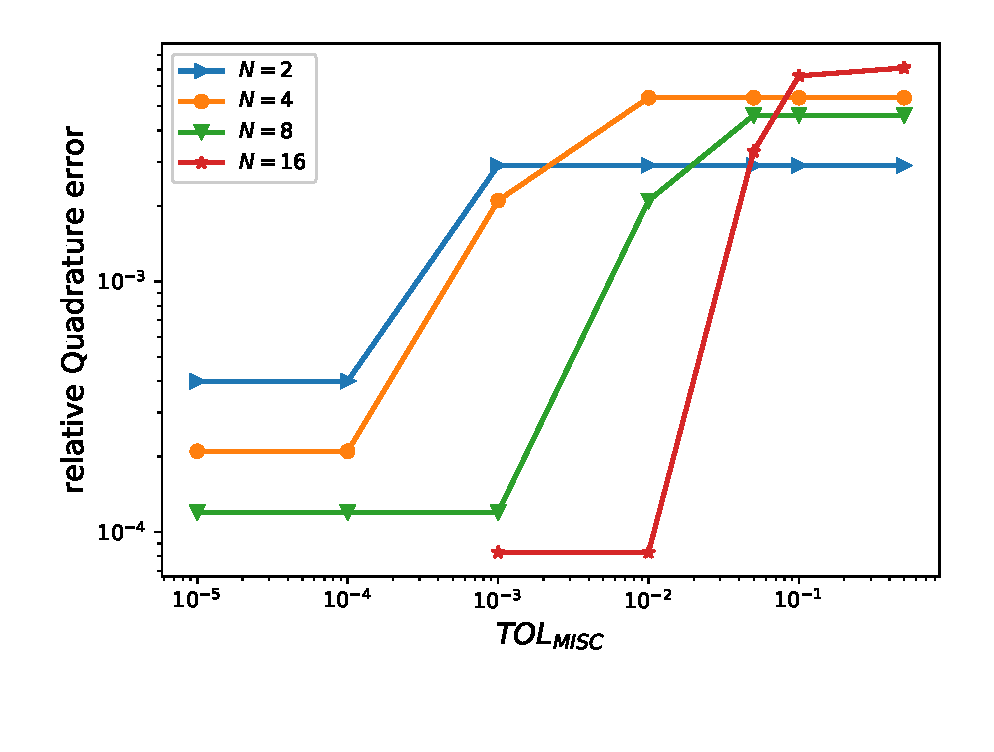
\includegraphics[width=0.35\linewidth]{./figures/rBergomi_MISC_quadratre_error/vs_TOL/set6/relative_quad_error_wrt_MISC_TOL_set6_non_rich}
%	
%	
%	\caption{Quadrature error of MISC, with different tolerances, to compute call option price  for different number of time steps. Case  set $3$ parameters, without Richardson extrapolation.}
%%	  See detailed values  in table \ref{Quadrature error of MISC to compute Call option price of the different tolerances for different number of time steps. Case  set $4$ parameters, without Richardson extrapolation. The numbers between parentheses are the corresponding absolute errors.}}
%	\label{fig:Quadrature_error_set4}
%\end{figure}
%
%
%
\FloatBarrier

\begin{table}[h!]
	\centering
	\begin{tabular}{l*{6}{c}r}
		Method \textbackslash  Steps            & $2$ & $4$ & $8$ & $16$  \\
		\hline

		MISC ($\text{TOL}_{\text{MISC}}=10^{-1}$)  &  $\underset{(0.006,0.002)}{\mathbf{0.008}}$ & $\underset{(0.004,0.005)}{\mathbf{0.009}}$& $\underset{(0.003,0.005)}{\mathbf{ 0.008}}$ & $\underset{(0.002,0.007)}{\mathbf{ 0.009}}$   \\

		MISC ($\text{TOL}_{\text{MISC}}=10^{-2}$)  &  $\underset{(0.006,0.002)}{\mathbf{0.008}}$ & $\underset{(0.004,0.005)}{\mathbf{0.009}}$& $\underset{(0.003,0.002)}{\mathbf{ 0.005}}$ & $\underset{(0.002,1e-04)}{\mathbf{ \red{0.002}}}$  \\
		MISC ($\text{TOL}_{\text{MISC}}=10^{-3}$)  &  $\underset{(0.006,0.002)}{\mathbf{0.008}}$& $\underset{(0.004,0.002)}{\mathbf{0.006}}$& $\underset{(0.003,1e-04)}{\mathbf{\red{0.003}}}$  & $\underset{(0.002,1e-04)}{\mathbf{ 0.002}}$  \\
		MISC ($\text{TOL}_{\text{MISC}}=10^{-4}$)  &  $\underset{(0.006,4e-04)}{\mathbf{\red{0.006}}}$ & $\underset{(0.004,2e-04)}{\mathbf{\red{0.004}}}$& $\underset{(0.003,1e-04)}{\mathbf{0.003}}$ & $\mathbf{ -}$ \\

		
		\hline
		MC    & $\underset{(0.006,4e-04)}{\mathbf{0.006}}$  & $\underset{(0.004,4e-04)}{ \mathbf{0.004}}$  & $\underset{(0.003,4e-04)}{\mathbf{0.003}}$ & $\underset{(0.002,4e-04)}{\mathbf{0.002}}$  \\	
		M(\# MC samples) 	& $5 \times 10^6$  & $5 \times 10^6$  & $5 \times 10^6$ & $5 \times 10^6$  \\
		\hline
	\end{tabular}
	\caption{Total relative error of MISC, without Richardson extrapolation, with different tolerances, and MC to compute call option price  for different number of time steps.}
	\label{Total error of MISC and MC to compute Call option price of the different tolerances for different number of time steps. Case set 4, without Richardson extrapolation. The numbers between parentheses are the corresponding absolute errors.}
\end{table}

\FloatBarrier
\begin{table}[h!]
	\centering
	\begin{tabular}{l*{6}{c}r}
		Method \textbackslash  Steps            & $2$ & $4$ & $8$ & $16$ &   \\
		\hline
%		MISC ($\text{TOL}_{\text{MISC}}=5.10^{-1}$)  & $0.1$ & $0.1$ & $0.1$ & $0.3$  \\
		MISC ($\text{TOL}_{\text{MISC}}=10^{-1}$)  & $0.1$ & $0.1$ & $0.1$ & $1$ \\
%		MISC ($\text{TOL}_{\text{MISC}}=5.10^{-2}$)  & $0.1$ & $0.1$ & $0.1$ & $22$  \\
		MISC ($\text{TOL}_{\text{MISC}}=10^{-2}$)  & $0.1$ & $0.15$ & $9$ & $\red{112}$ \\
		MISC ($\text{TOL}_{\text{MISC}}=10^{-3}$)  & $0.2$ & $2$ & $\red{27}$ & $2226$ \\
		MISC ($\text{TOL}_{\text{MISC}}=10^{-4}$)  & $\red{1}$ & $\red{6}$ & $136$ & $-$\\
%		MISC ($\text{TOL}_{\text{MISC}}=10^{-5}$)  & $2$ & $18$ & $1559$ & $-$
%		\\
		\hline
		MC method   & $ \red{141}
		
		$  & $  \red{246}$  & $  \red{461}$ & $ \red{820}
		$  \\	
		\hline
		Ratio of CPU time  $\left(MC/MISC \right)$ & $ \red{141}
		
		$  & $  \red{
			41
		}$  & $  \red{    17
		}$ & $ \red{ 7}
		$  \\	
%		
		\hline
	\end{tabular}
	\caption{Comparison of the computational time (in Seconds) of  MC and MISC, used to compute call option price of the rBergomi model for different number of time steps. The average  MC CPU time is computed over $10$ runs. }
	\label{Comparsion of the computational time of  MC and MISC, used to compute Call option price of rBergomi model for different number of time steps. Case set4}
\end{table}


\FloatBarrier

	\begin{figure}[h!]
	\centering
	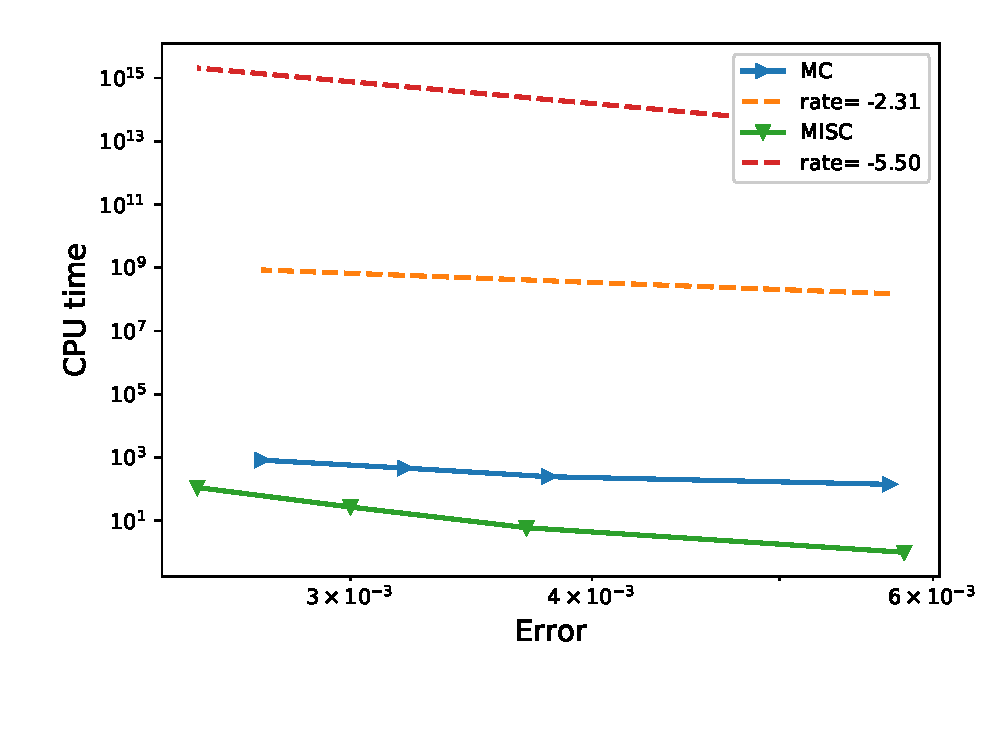
\includegraphics[width=0.5\linewidth]{./figures/rBergomi_Complexity_rates/set6/error_vs_time_set6}
	
	\caption{Comparison of computational work for MC and MISC.}
	\label{fig:Complexity plot for MC and MISC for case set $4$ parameters}
\end{figure}
\FloatBarrier
\subsubsection{Case of set $4$ parameters in Table \ref{table:Reference solution, using MC with $500$ time steps, of Call option price under rBergomi model, for different parameter constellation.}}\label{sec:Case of set 5 parameters}

For the case of set $4$, we just conduct our numerical experiments for the case without Richardson extrapolation. Our numerical experiments show that  MISC is  $220$ times faster than MC, to achieve a total relative error below $7\%$ and $16$ times faster than MC, to achieve a total relative error around $2\%$  (see Figure \ref{fig:Complexity plot for MC and MISC for Case set $5$ parameters} and Tables \ref{Comparsion of the computational time of  MC and MISC, used to compute Call option price of rBergomi model for different number of time steps. Case set5} and \ref{Total error of MISC and MC to compute Call option price of the different tolerances for different number of time steps. Case set 5, without Richardson extrapolation. The numbers between parentheses are the corresponding absolute errors.}).

%\FloatBarrier
%\begin{table}[h!]
%	\centering
%	\begin{tabular}{l*{6}{c}r}
%		Method \textbackslash  Steps            & $2$ & $4$ & $8$ & $16$ &   \\
%		\hline
%%		MISC ($\text{TOL}_{\text{MISC}}=5.10^{-1}$)  & $0.0590$ & $0.0564$ & $0.0552$ & $0.0546$  \\
%		MISC ($\text{TOL}_{\text{MISC}}=10^{-1}$)  & $0.0590$ &$0.0564$& $0.0552$ & $0.0546$   \\
%%		MISC ($\text{TOL}_{\text{MISC}}=5.10^{-2}$)  &$0.0590$ & $0.0564$ & $0.0552$ & $0.0557$  \\
%		MISC ($\text{TOL}_{\text{MISC}}=10^{-2}$)  &$0.0590$ &$0.0564$ & $0.0574$ & $0.0572$  \\
%		
%		MISC ($\text{TOL}_{\text{MISC}}=10^{-3}$)  & $0.0605$ & $0.0587$ & $0.0579$ & $0.0575$  \\
%%		MISC ($\text{TOL}_{\text{MISC}}=10^{-4}$)  &  $0.0605$ & $0.0587$ & $0.0576$ & $-$  \\
%%		
%%		MISC ($\text{TOL}_{\text{MISC}}=10^{-5}$)  & $0.0605$ & $0.0587$ &  $0.0579$ & $-$  \\
%		\hline
%		MC method ($M=5.10^{6}$)   & $0.0605$ & $0.0587$  & $0.0579$ & $0.0576$ \\		
%		
%		\hline
%	\end{tabular}
%	\caption{ Call option price of the different methods for different number of time steps. Case of set $5$ parameters in table \ref{table:Reference solution, using MC with $500$ time steps, of Call option price under rBergomi model, for different parameter constellation.}, without Richardson extrapolation.}
%	\label{table: Call option price of the different methods for different number of time steps. Case set 5}
%\end{table}

%\FloatBarrier
%\begin{table}[h!]
%	\centering
%	\begin{tabular}{l*{6}{c}r}
%		Method \textbackslash  Steps            & $2$ & $4$ & $8$ & $16$  \\
%		\hline
%		MC Bias ($M=5.10^6$)   & 	$ \underset{(0.0037
%			)}{\mathbf{0.0650}}$  & $\underset{(0.0019)}{\mathbf{0.0330
%		}}$  & $\underset{(0.0012)}{\mathbf{0.0202}}$ & $\underset{(0.0007)}{\mathbf{0.0130}}$\\ 
%		
%		MC Statistical error ($M=5.10^6$)  &  $\underset{(   4.0e-05)} {\mathbf{7.0e-04}}$  & $\underset{(3.8e-05)} {\mathbf{6.7e-04}}$  & $\underset{(3.7e-05)} {\mathbf{6.5e-04 }}$ & $\underset{(3.6e-05)} {\mathbf{6.3e-04}}$	\\
%		
%		\hline
%	\end{tabular}
%	\caption{Bias and statistical errors of MC   for computing call option price  for different number of time steps. Case set $4$, without Richardson extrapolation. The numbers between parentheses are the corresponding absolute errors.}
%	\label{Bias and Statistical errors of MC ($M=5.10^6$)  for computing Call option price  for different number of time steps. Case set 5, without Richardson extrapolation. The numbers between parentheses are the corresponding absolute errors.}
%\end{table}
%%
%%
%%
%
%
%\FloatBarrier





%\begin{figure}[h!]
%	\centering
%	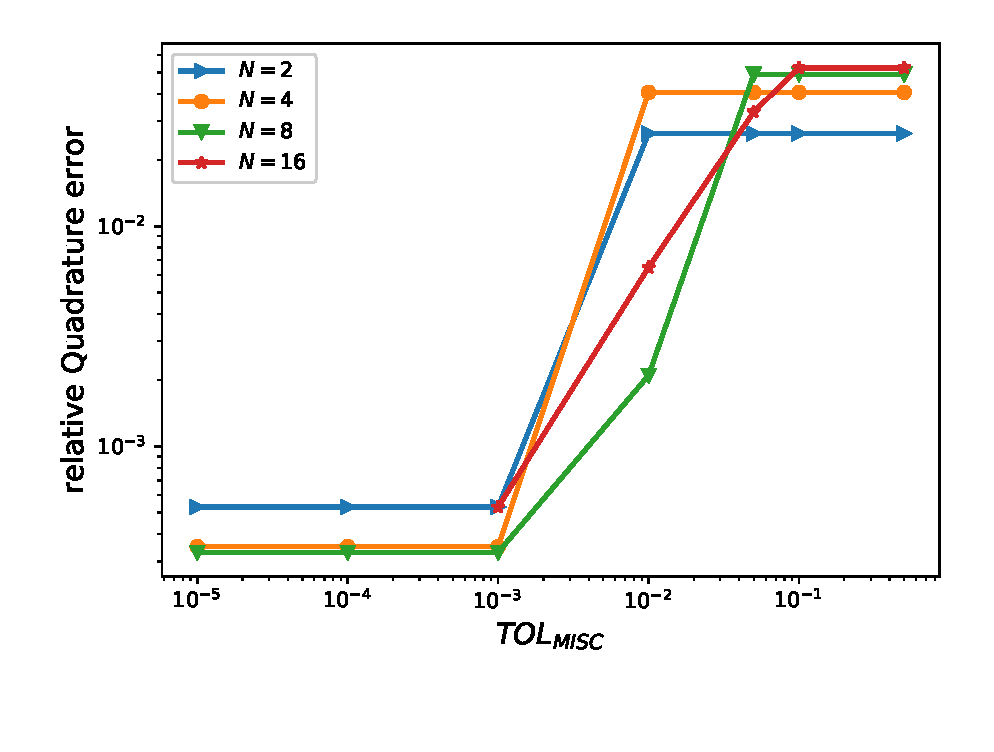
\includegraphics[width=0.35\linewidth]{./figures/rBergomi_MISC_quadratre_error/vs_TOL/set7/relative_quad_error_wrt_MISC_TOL_set7_non_rich}
%	
%	
%	\caption{Quadrature error of MISC, with  different tolerances,  to compute call option price  for different number of time steps. Case  set $4$ parameters, without Richardson extrapolation. }
%%	 See detailed values  in table \ref{Quadrature error of MISC to compute Call option price of the different tolerances for different number of time steps. Case  set $5$ parameters, without Richardson extrapolation. The numbers between parentheses are the corresponding absolute errors.}}
%	\label{fig:Quadrature_error_set5}
%\end{figure}
%
%\FloatBarrier
%%
%
%
\begin{table}[h!]
	\centering
	\begin{tabular}{l*{6}{c}r}
		Method \textbackslash  Steps            & $2$ & $4$ & $8$ & $16$  \\
		\hline

		MISC ($\text{TOL}_{\text{MISC}}=10^{-1}$)  & $\underset{(0.07,0.05)}{\mathbf{0.09}}$ & $\underset{(0.03,0.04)}{\mathbf{0.07}}$& $\underset{(0.02,0.05)}{\mathbf{ 0.07}}$ & $\underset{(0.01,2e-04)}{\mathbf{ 0.06}}$   \\

		MISC ($\text{TOL}_{\text{MISC}}=10^{-2}$)  &  $\underset{(0.07,5e-04)}{\mathbf{0.09}}$& $\underset{(0.03,0.04)}{\mathbf{0.07}}$& $\underset{(0.02,3e-04)}{\mathbf{ 0.02}}$ & $\underset{(0.01,2e-04)}{\mathbf{ 0.02}}$  \\
		MISC ($\text{TOL}_{\text{MISC}}=10^{-3}$)  &  $\underset{(0.07,5e-04)}{\mathbf{\red{0.07}}}$& $\underset{(0.03,4e-04)}{\mathbf{\red{0.03}}}$& $\underset{(0.02,3e-04)}{\mathbf{\red{0.02}}}$  & $\underset{(0.01,2e-04)}{\mathbf{ \red{0.01}}}$  \\

		\hline
		MC    & $\underset{(0.07,7e-04)}{\mathbf{0.07}}$  & $\underset{(0.03,6e-04)}{\mathbf{0.03}}$  & $\underset{(0.02,6e-04)}{\mathbf{0.02}}$ & $\underset{(0.01,6e-04)}{\mathbf{0.01}}$  \\		
			M(\# MC samples)   & $5 \times 10^6$  & $5 \times 10^6$  & $5 \times 10^6$ & $5 \times 10^6$  \\		
		\hline
	\end{tabular}
	\caption{Total relative error of MISC, without Richardson extrapolation, with  different tolerances,  and MC to compute call option price  for different number of time steps.}
	\label{Total error of MISC and MC to compute Call option price of the different tolerances for different number of time steps. Case set 5, without Richardson extrapolation. The numbers between parentheses are the corresponding absolute errors.}
\end{table}

\FloatBarrier
\begin{table}[h!]
	\centering
	\begin{tabular}{l*{6}{c}r}
		Method \textbackslash  Steps            & $2$ & $4$ & $8$ & $16$ &   \\
		\hline
%		MISC ($\text{TOL}_{\text{MISC}}=5.10^{-1}$)  & $0.1$ & $0.1$ & $0.2$ & $0.5$  \\
		MISC ($\text{TOL}_{\text{MISC}}=10^{-1}$)  & $0.1$ & $0.1$ & $0.2$ & $0.5$ \\
%		MISC ($\text{TOL}_{\text{MISC}}=5.10^{-2}$)  & $0.1$ & $0.1$ & $0.2$ & $5$  \\
		MISC ($\text{TOL}_{\text{MISC}}=10^{-2}$)  & $0.1$ & $0.1$ & $8$ & $97$ \\
		MISC ($\text{TOL}_{\text{MISC}}=10^{-3}$)  & $\red{0.7}$ & $\red{4}$ & $\red{26}$ & $\red{1984}$ \\
%		MISC ($\text{TOL}_{\text{MISC}}=10^{-4}$)  & $1$ & $8$ & $173$ & $-$\\
%		MISC ($\text{TOL}_{\text{MISC}}=10^{-5}$)  & $1$ & $32$ & $2129$ & $-$
%		\\
		\hline
		MC method   & $ \red{154}
		
		$  & $  \red{229}$  & $  \red{420}$ & $ \red{938}
		$  \\	
		\hline
		Ratio of CPU time  $\left(MC/MISC \right)$ & $ \red{   220}
		
		$  & $  \red{
		 57
		}$  & $  \red{    16
		}$ & $ \red{ 0.5}
		$  \\	
				
		\hline
	\end{tabular}
	\caption{Comparison of the computational time (In seconds) of  MC and MISC, used to compute call option price of rBergomi model for different number of time steps. The average  MC CPU time is computed over $10$ runs. }
	\label{Comparsion of the computational time of  MC and MISC, used to compute Call option price of rBergomi model for different number of time steps. Case set5}
\end{table}

\FloatBarrier


	\begin{figure}[h!]
	\centering
	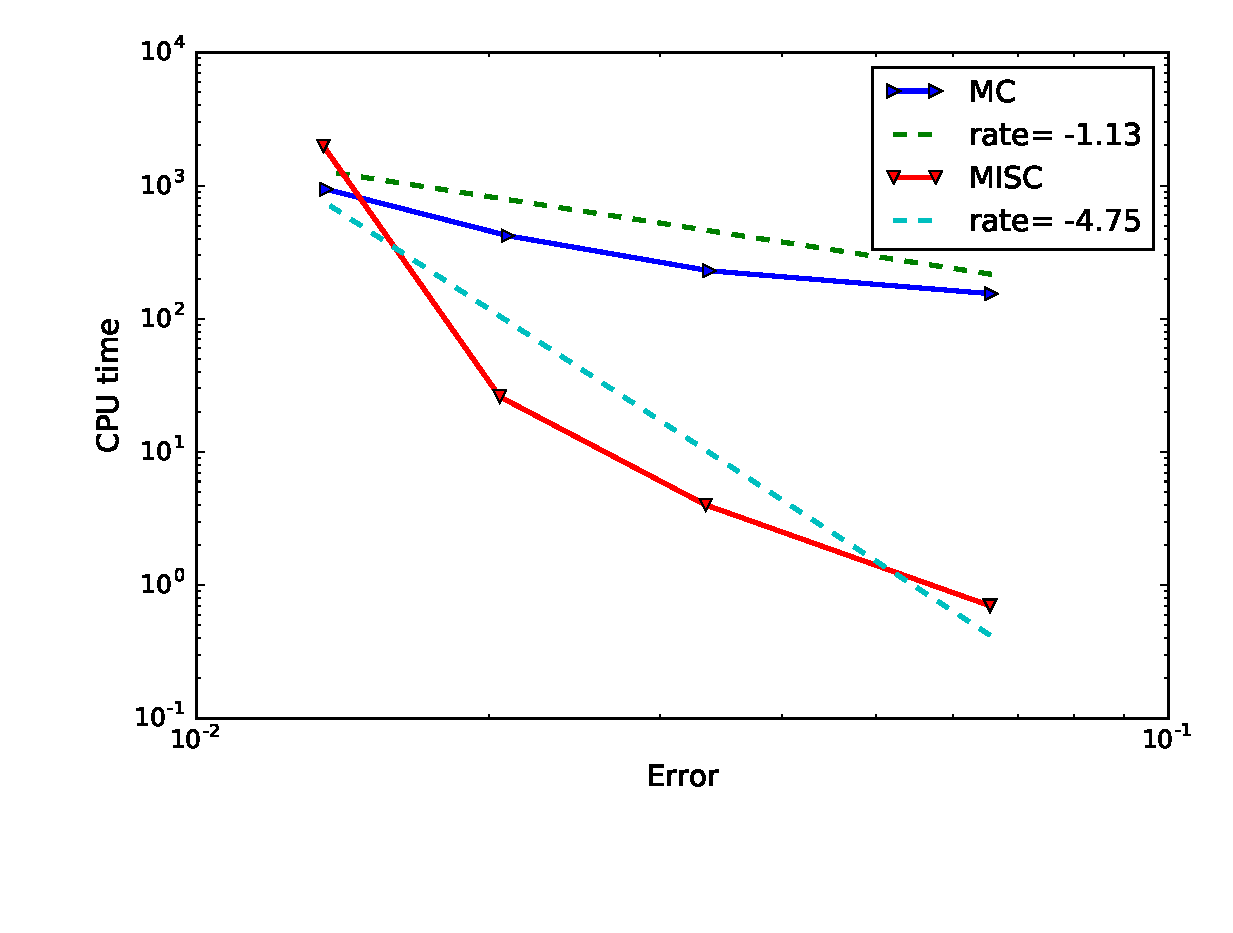
\includegraphics[width=0.5\linewidth]{./figures/rBergomi_Complexity_rates/set7/error_vs_time_set7}
	
	\caption{Comparison of computational work for MC and MISC.}
	\label{fig:Complexity plot for MC and MISC for Case set $5$ parameters}
\end{figure}
\FloatBarrier
}


